% Get rid of some pdf warnings
\pdfminorversion=7

% DAIM example scaled to A4 (slightly smaller text and thus less pages)
\documentclass[a4paper,twoside,12pt]{book}
\usepackage[left=30mm,right=30mm,top=32mm,bottom=36mm]{geometry}

\usepackage[utf8]{inputenc} % UTF-8
\usepackage[T1]{fontenc} % 8-bit fonts

\usepackage{parskip} % Linebreaks between paragraphs
\usepackage{pdfpages} % PDF includes

\usepackage{lmodern} % Modern font

\usepackage{xcolor} % Colors
\usepackage{hyperref} % URLs
\usepackage{graphicx} % Graphics
\usepackage{rotating} % Rotated graphics

\usepackage{booktabs} % Formal tables
\usepackage{multirow} % Table cells that span multiple rows
\usepackage{colortbl} % Table cell coloring

\usepackage{subcaption} % Subfigures

\usepackage{tabularx} % Better tables
\usepackage{array} % Used to align in tables

\usepackage{dirtree} % Directory trees

\usepackage{siunitx}

\usepackage{verbatim}
\usepackage{listings}
\lstset{
    columns=flexible,
    basicstyle={\small\ttfamily},
    numbers=left,
    numberstyle={\tiny\color{gray}}
}
\graphicspath{{figures/}}

\hypersetup{
    colorlinks,
    linkcolor={red!40!black},
    citecolor={blue!40!black},
    urlcolor={blue!80!black}
}

\newcommand\TODO{\textcolor{red}{[TODO]}}
\newcommand\todo[1]{\textcolor{red}{[TODO: #1]}}
\newcommand\CN{\textcolor{blue}{[Citation Needed]}}
\newcommand\cn[1]{\textcolor{blue}{[Citation Needed: #1]}}

% Size of a block in LucidChart
\newlength{\block}
\setlength{\block}{0.02\textwidth}

\title{
    {The Cellular Automata Research Platform}\\
    \TODO
}
\author{Per Thomas Lundal}
\date{2015-06-14}

\begin{document}

\maketitle

% Add blank page after title (since two-sided)
% Unknown why it is not created automatically
\clearpage
\null
\pagenumbering{gobble}
\newpage

\pagenumbering{roman}

\cleardoublepage
\phantomsection
\addcontentsline{toc}{chapter}{Sammendrag}
\chapter*{Sammendrag}
    \TODO

\cleardoublepage
\phantomsection
\addcontentsline{toc}{chapter}{Abstract}
\chapter*{Abstract}
    Nature has many attractive properties that engineers hope to once incorporate into man-made technology to revolutionize computing.
Properties include, among other things, reproduction, learning, adaption and massive parallelism.
One bio-inspired computational structure is the Cellular Automaton (CA), which can mimic the massively parallel, distributed and locally interactive nature of multi-cellular organisms.

At NTNU, three master theses have gone into creating a Field-Programmable Gate Array (FPGA) platform whose purpose is to allow research on CAs in combination with artificial evolution and development.
The main principle is that a Genetic Algorithm (GA) is used to create development rules, which are then used to build a CA, which can finally be used to compute a fitness value.
The fitness value is then fed back fed into the GA and the process is repeated until a good solution is found.

In expectation of new hardware with a larger FPGA, the purpose of most recent thesis was to take advantage of increased resources to improve speed and to extend the CA into 3D.
However, the hardware failed to be delivered on time due to manufacturing problems.
This caused the new communication module to remain unimplemented and only allowed rudimentary simulation testing.

In a specialization project leading up to this thesis, a new communication module was implemented and integrated into the platform, allowing proper hardware verification.
It showed that the design had many issues, including failing instructions, extensive use of outdated features and separate versions for 2D and 3D CAs.
In this thesis, the entire platform has therefore been revised and rebuilt.

The new platform solves all major issues with the previous and adds further enhancements such as more advanced control flow and an adaptive software API.
More and better fine-tunable build parameters allow wider adjustment of performance and make it possible to fit larger CAs within the FPGA.

The functionality of all instructions is verified in hardware and a program that creates replicating structures is demonstrated, proving that the platform is complete and ready to be used for research.
A clocking issue with the communication module is currently reducing the entire platform to half speed, but if fixed, the raw CA performance will be 35\% higher in 2D and 300\% higher in 3D compared to the previous design.
For those performance configurations, resource usage is significantly lower in 2D and equivalent in 3D.


\cleardoublepage
\phantomsection
\addcontentsline{toc}{chapter}{Preface}
\chapter*{Preface}
    This master's thesis has been conducted at the Department of Computer and Information Science at the Norwegian University of Science and Technology under supervision of Associate Professor Gunnar Tufte.

The thesis counts for 30 credits and is the continuation of a 15-credit specialization project conducted autumn 2014.
It concludes a 5-year master of science study in Computer Science.

I would like to personally thank Gunnar Tufte for his invaluable inspiration and support, and Odd Rune Strømmen Lykkebø who stepped in during his brief absence.

\vspace{\fill}

\begin{flushright}
Per Thomas Lundal
\\
2015 June 14th
\end{flushright}


\setcounter{tocdepth}{2}

\cleardoublepage
\phantomsection
\addcontentsline{toc}{chapter}{\contentsname}
\tableofcontents

\cleardoublepage
\phantomsection
\addcontentsline{toc}{chapter}{\listfigurename}
\listoffigures

\cleardoublepage
\phantomsection
\addcontentsline{toc}{chapter}{\listtablename}
\listoftables

\cleardoublepage
\pagenumbering{arabic}

\chapter{Introduction}
    \label{ch:introduction}
    \TODO

The initial work was done by Dupdal, and was promptly extended by Aamodt.

\section{Motivation}

\todo{maybe not separate section}

\begin{itemize}
    \item Fix all instructions
    \item More modular and maintainable
    \item More configurable (not only powers of two)
    \item Better resource utilization
    \item Adaptive API
    \item Simpler build system
    \item More advanced control flow
    \item Toggle matrix wrapping
    \item Remove outdated code (tristates and reset)
    \item Data structures instead of prints in API
\end{itemize}

\section{Outline}

\TODO
The thesis is organized as follows:

\begin{itemize}
    \item Chapter \ref{ch:background} –
        Theoretical background, technology and related work.
        This chapter gives an overview of the relevant research this thesis is based on and the technology which is used.
    \item Chapter \ref{ch:previous-work} –
        \TODO
    \item Chapter \ref{ch:development-platform} –
        \TODO
    \item Chapter \ref{ch:implementation} –
        Implementation details.
        This chapter provides in-depth details of all parts of the rebuilt and extended platform.
        \TODO
    \item Chapter \ref{ch:verification} –
        \TODO
    \item Chapter \ref{ch:discussion} –
        \TODO
    \item Chapter \ref{ch:conclusion} –
        Concluding remarks.
        The final chapter concludes this paper by reviewing the new platform, its performance and its potential for future applications.
    \item Appendices –
        \TODO
\end{itemize}


\chapter{Background}
    \label{ch:background}
    \TODO

\begin{itemize}
    \item EHW
    \item POE
\end{itemize}

\section{Artificial Evolution}

\TODO

\begin{itemize}
    \item Antenna design
    \item Robot controllers
\end{itemize}

\subsection{Genetic Algoritmhs}

\TODO

\begin{itemize}
    \item Select, Cross, Mutate
    \item Genotype to Phenotype
\end{itemize}

\subsection{Evolution in Materio}

\TODO

\section{Artificial Development}

\TODO

\begin{itemize}
    \item Attractors
    \item Adaptation
    \item Graceful degradation
\end{itemize}

\subsection{Lindenmayer Systems}

\TODO

\section{Cellular Automata}

\TODO

\begin{itemize}
    \item 1D, 2D, 3D
    \item Neighborhoods
    \item Wolfram's classes
\end{itemize}

\section{FPGA}

\TODO

\section{PCI Express}

The PCI Express interface was designed to tackle the arising trouble with clocked parallel buses like PCI.
The problem with such buses is that the clock speed can not be increased beyond a given threshold, as the slightly different lengths of the wires causes data to arrive at slightly different times.
Reducing the clock period to less than the variation in arrival time means the data will become corrupted.
This problem is exacerbated with increasing bus size.

PCI Express is therefore based on serial communication over differential pairs (lanes\footnotemark) without the need for a reference clock \cite{pcie}.
\footnotetext{
    PCI Express operates in full duplex mode, which means that each lane has an independent differential pair in each direction.
    1, 2, 4, 8, 16 or 32 lanes are supported, but data is striped and thus still transmitted serially.
}
This allows an extremely fast clock speed compared to a parallel bus, and much greater bandwidth in total.
PCI Express consists of three layers; the physical layer, the data link layer and the transaction layer, structured as shown in \figurename~\ref{fig:pcie}.

\begin{figure}[!ht]
    \centering
    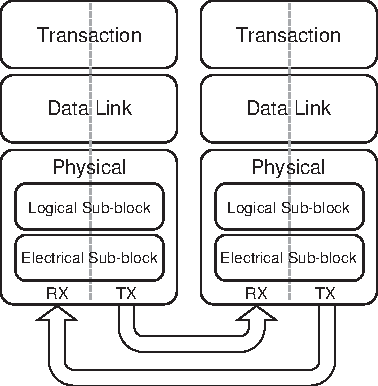
\includegraphics[width=0.5\textwidth]{pcie}
    \caption[PCI Express structure]{
        High-level diagram showing the layered structure of PCI Express. (Reprinted from \cite{pcie})
    }
    \label{fig:pcie}
\end{figure}

The transaction layer's primary responsibility is the creation and parsing of transaction layer packets (TLPs).
TLPs are used to trigger events or start various transactions, most commonly to initiate read and write requests\footnotemark.
\footnotetext{
    Read and write requests are directed at one of up to six base address registers (BARs).
    They represent internal memory areas that can be anywhere from a few bytes to several gigabytes in size.
}
Most requests entail the return of a completion TLP containing the requested data or other information.
TLPs consists of multiple 32-bit double words (DW), where the first is a common header describing the type of packet.

The data link layer ensures integrity by adding error detection codes to outgoing TLPs and performing error detection and correction on incoming TLPs.
It is also responsible for retransmission if corruption occurs.

The physical layer is responsible for serialization and deserialization of the data stream.
Each byte is padded with two extra bits (8b/10b encoding) to allow clock recovery.

\section{Related Work}

\TODO

\subsection{CAM-Brain Machine}

\TODO

\subsection{CAM-8}

\TODO


\chapter{Previous Work}
    \label{ch:previous-work}
    This thesis continues to build on the Cellular Automata Research Platform (CARP), which is the result of three previous master theses at NTNU.
The original implementation was made by Djupdal in 2003.
It was then extended with a range of various output methods by Aamodt in 2005.
Finally, it was further extended and optimized in expectation of new hardware by Støvneng in 2014.

\begin{figure}[!ht]
    \centering
    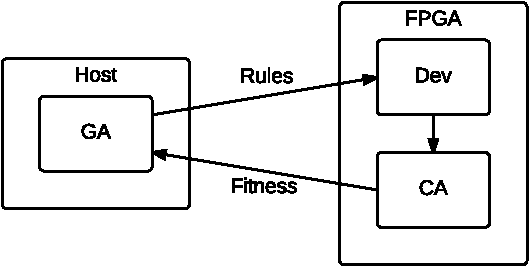
\includegraphics[width=28\block]{figures/overview-general}
    \caption[System design]{
        General system design.
    }
    \label{fig:overview-general}
\end{figure}

The platform is more or less a ``proof of principle'' for how a CA can be combined with development and evolution to create a powerful bio-inspired system.
The general system design, which is based on the setup in Section~\ref{sec:evo-devo-ca}, is depicted in \figurename~\ref{fig:overview-general}:
An FPGA implements the CA and development process while evolution is performed by a host computer.

%==============================================================================%

\section{Djupdal}

In 2002, NTNU invested in a CompactPCI computer with a NallaTech BenERA FPGA board to be used for research within the field of evolutionary hardware.
The task of developing a platform for the system, based on a matrix of sblocks, fell to Djupdal \cite{djupdal2003sblock}.

An overview of the resulting hardware platform is shown in \figurename~\ref{fig:overview-djupdal}.
It consists of the mentioned sblock matrix, block RAM (BRAM) for storing the state and type of each cell, a development unit, control logic, and a PCI communication unit.

\begin{figure}[!ht]
    \centering
    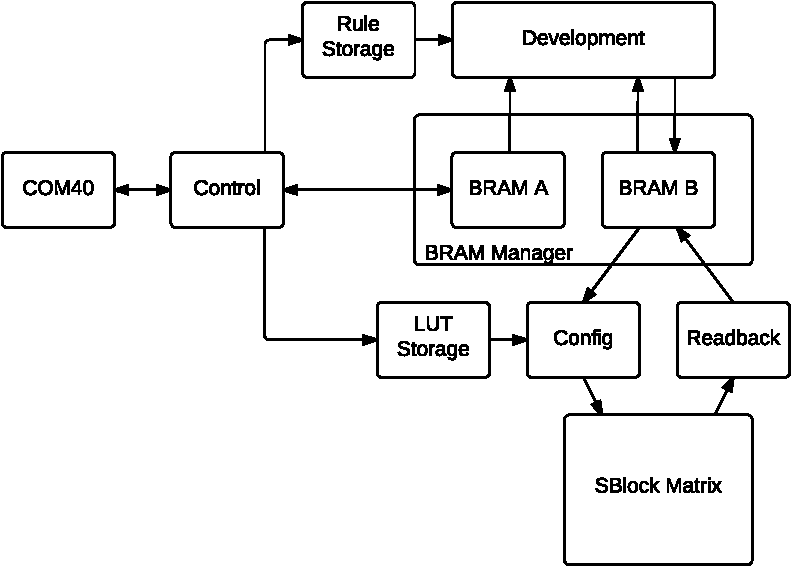
\includegraphics[width=42\block]{figures/overview-djupdal}
    \caption[Djupdal's hardware design]{
        High-level block diagram of the hardware platform after Djupdal's original work.
    }
    \label{fig:overview-djupdal}
\end{figure}

The system is meant to be controlled by a computer running a genetic algorithm.
A common flow of operation is to initialize the system with the genotype, develop it into its phenotype, run the SBM, and send the new states back to the computer.
The computer then uses the newly received state data to calculate a fitness score.

The system is initialized by writing states and types to BRAM A, in addition to storing development rules and LUT conversion rules.
Then a development step can be performed by reading cell types from BRAM A\footnotemark, testing development rules, and writing the (possibly changed) types back to BRAM B.
\footnotetext{
    After the first 8 rules have been tested on all cells, center cell types are read from BRAM B instead.
    This is needed to prevent the result of a rule in an earlier iteration from being deleted if no rules trigger in a later iteration.
}
The development unit tests 8 rules on 2 cells each cycle in raster order.
Optionally, the BRAMs can be logically swapped and further development steps performed.
The SBM can then be configured by translating the types in BRAM B into LUT entries according to the LUT conversion rules, before being run for a desired amount of cycles.
Afterwards, the new states in the SBM can be read back into BRAM B, swapped into BRAM A, and sent to the computer.

The design is split into two clock domains; the communication unit uses 40 MHz to be able to interface with PCI, while the rest uses 80 MHz for higher performance.

%==============================================================================%

\section{Aamodt}

There was one major bottleneck in the original design.
To calculate the fitness of an individual, the state of each cell had to be transferred to the computer over the PCI interface.
Having a dedicated hardware unit would greatly improve the performance.
Additionally, it was desired to have more information about the development process.
The task of realizing this fell to Aamodt \cite{aamodt2005sblock}.

An overview of the hardware platform with Aamodt's additions is shown in \figurename~\ref{fig:overview-aamodt}.
The additions consists of a Run-Step Function (RSF) that calculates the number of live cells, BRAM to store the numbers, a fitness function, and two information outputs from the development unit.

\begin{figure}[!ht]
    \centering
    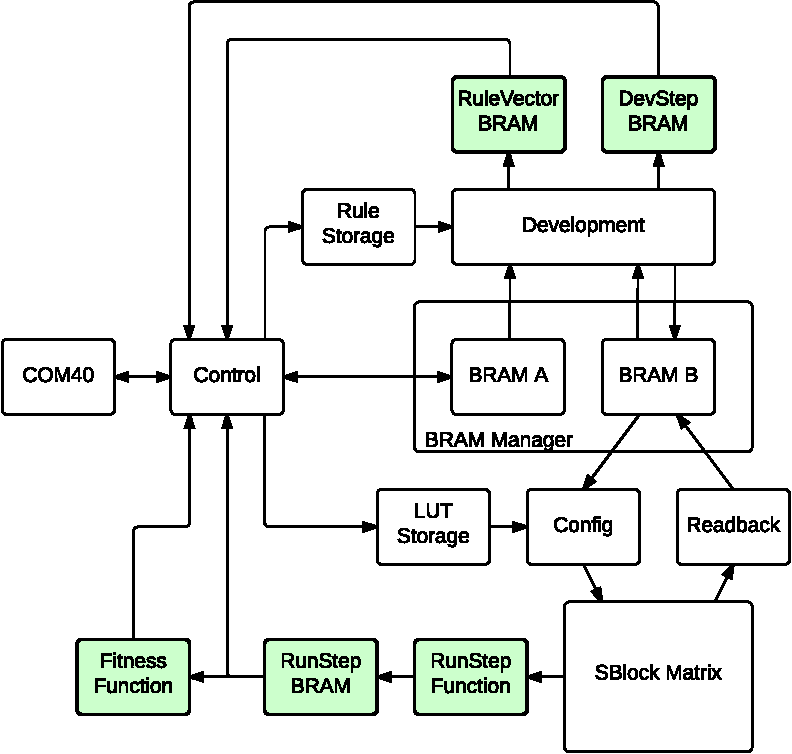
\includegraphics[width=42\block]{figures/overview-aamodt}
    \caption[Aamodt's hardware design]{
        High-level block diagram of the hardware platform after Aamodt's work.
        Additions are highlighted in green.
    }
    \label{fig:overview-aamodt}
\end{figure}

The rule vector BRAM stores lists of which rules were triggered and not for the last 256 development steps.
The lists are implemented as bit-vectors where each bit represents the status of a rule for a single development step.
The development step BRAM is more detailed; it stores which rule was triggered for each cell.
However, it only has storage space for one development step.

The run-step function calculates the number of live cells after each SBM update by using a large adder tree.
The numbers are stored in run-step BRAM for later usage by the fitness function, which is replaceable.

%==============================================================================%

\section{Støvneng}

In expectation of receiving new hardware with a larger and faster FPGA, there was a demand to optimize the platform by taking advantage of the increased resource pool.
Extending the platform into the third dimension was also a lucrative thought, as doing so allows more complex signal pathways to form within the cellular automata.
It was also desired to have a Discrete Fourier Transform (DFT) for interpretation of the RSF data; it should give very useful data according to Berg's research \cite{berg2013ca}.
The task of realizing this was taken on by Støvneng \cite{stovneng2014sblock}.

\begin{figure}[!ht]
    \centering
    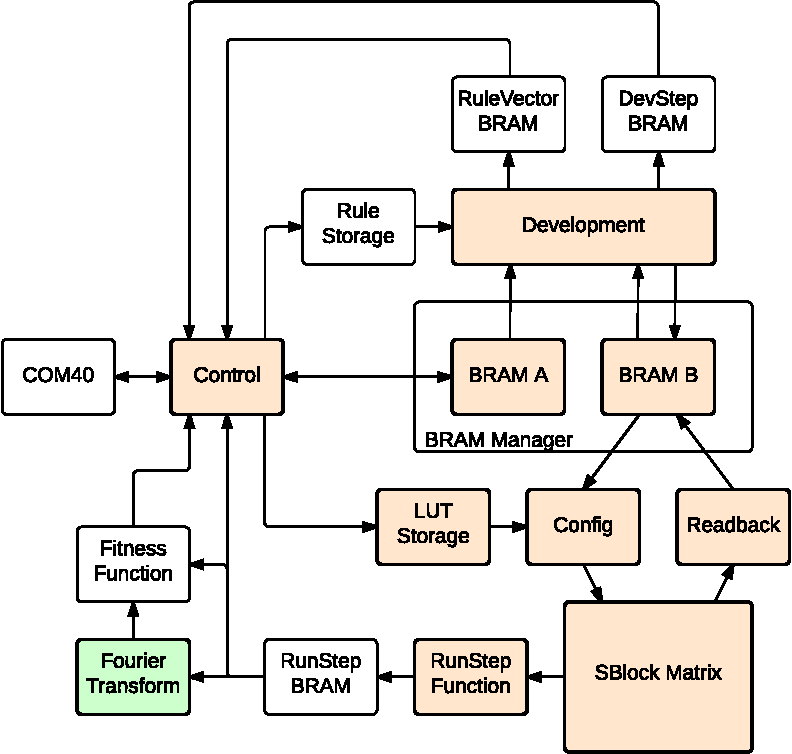
\includegraphics[width=42\block]{figures/overview-stovneng}
    \caption[Støvneng's hardware design]{
        High-level block diagram of the hardware platform after Støvneng's work.
        Additions are highlighted in green, and optimizations and 3D modifications in orange.
    }
    \label{fig:overview-stovneng}
\end{figure}

An overview of the hardware platform with Støvneng's additions and optimizations is shown in \figurename~\ref{fig:overview-stovneng}.
The only addition is the DFT, but nearly all units has been optimized, yielding a speedup of 4 for most operations.

Unfortunately, due to some challenges with manufacturing, Støvneng was unable to get hold of the new hardware for the duration of his project.
The system was therefore only verified in simulation, and the PCI communication unit was not upgraded for the PCI Express connection on the new board.

%==============================================================================%

\section{Issues}

The original idea was to complete Støvneng's design by implementing the PCI Express module and driver in the specialization project leading up to this thesis, and then proceed to use the platform for research.
However, after successful integration, verification of the platform revealed multiple serious issues, which are listed in Table~\ref{tab:issues}.
The full project report can be read in Appendix~\ref{app:specialization-project}.

\begin{table}[!ht]
    \renewcommand{\arraystretch}{1.3}
    \centering
    \begin{tabular}{l|l}
        \bfseries Type & \bfseries Issue \\
        \hline
        Severe & Many instructions fail or do not follow specification \\
        Severe & The code is unnecessarily complex, making debugging nearly impossible \\
        Minor & Outdated features are extensively used (tristate buffers and global resets) \\
        Minor & Two different hardware designs and software APIs (2D and 3D) \\
        Minor & DFT twiddle factors are generated by an external python program \\
        Minor & It is impossible to retrieve the hardware parameters in the software API \\
        Minor & There is almost no control flow available in the hardware design \\
    \end{tabular}
    \caption[Issues]{Issues with the existing design.}
    \label{tab:issues}
\end{table}

Starting from a blank slate would allow the platform to be made more modular, more configurable, and more maintainable.
Also, it would be possible to unify the 2D and 3D designs and remove external dependencies.
This led to the decision of rebuilding the entire platform from scratch.


\chapter{Development Platform}
    \label{ch:development-platform}
    \TODO
Hoped for a chip with Spartan-6 LX145T (Støvneng planned for it).
Could not be delivered.
Got SP605 with LX45T instead.
Same architecture, 70\% less logic.
Scalable: Can simply reduce size of sblock matrix.

\section{Spartan-6 SP605 Evaluation Platform}

The Spartan-6 SP605 Evaluation Platform is essentially a board with the Spartan-6 LX45T FPGA wired to every useful peripheral imaginable.
It has connections for PCI Express\footnotemark, ethernet, DVI, USB, flash card, JTAG, LEDs, switches, and more.
However, the only peripherals utilized in this paper are PCI Express and JTAG.
An overview of the system is shown in \figurename~\ref{fig:sp605}.

\footnotetext {
    Even though the PCI Express finger has lines for power, they are not connected on the SP605.
    This means an external power source has to be connected.
}

\begin{figure}[!ht]
    \centering
    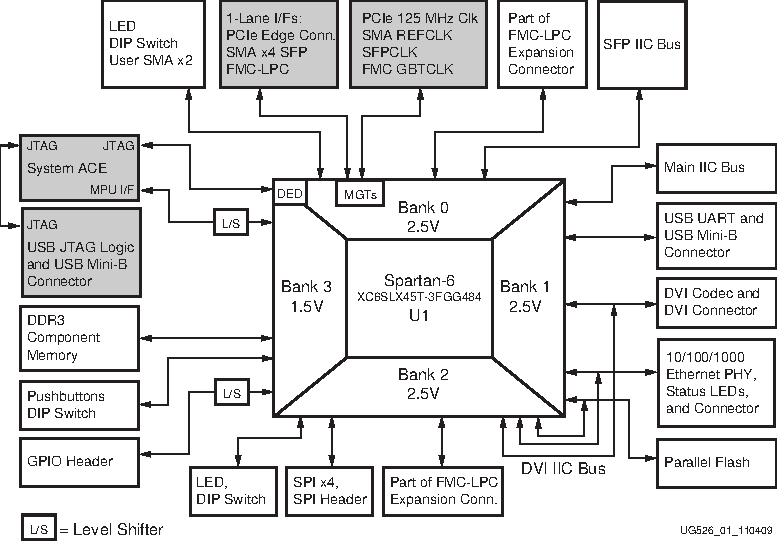
\includegraphics[width=\textwidth]{figures/sp605-modified}
    \caption[SP605]{
        High-level block diagram of the SP605 and its peripherals.
        Peripherals utilized in this paper are highlighted in gray.
        (Modified reprint from \cite{ug526})
    }
    \label{fig:sp605}
\end{figure}

The switch and jumper configurations of the SP605 are set to factory defaults per \cite{ug526}, with the exception of SW1 which is set to 10 (M0=1 and M1=0).

\section{Hardware Setup}

Due to the experimental nature of testing a new hardware platform, two computers were used in this project, as shown in \figurename~\ref{fig:hardware-setup}.
One is the main development workstation, used for coding and synthesis; it has a JTAG connection to the SP605 over USB, which allows it to upload new designs.
The other is the host for the SP605, which is mounted in a PCI Express expansion slot.

\begin{figure}[!ht]
    \centering
    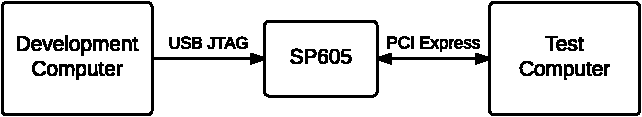
\includegraphics[width=0.70\textwidth]{figures/hardware-setup}
    \caption[Hardware setup]{
        High-level block diagram of the hardware setup.
    }
    \label{fig:hardware-setup}
\end{figure}

The setup allows a new design to be uploaded and tested on the SP605 without disrupting the workflow of the main workstation due to the power-cycle required to reset the PCI Express connection after a new design has been uploaded.

\section{Software Setup}

The operating systems used on the computers have varied, without complications, between Linux Mint 16, Linux Mint 17 and Manjaro during the lifespan of the project.
Linux Mint and Ubuntu, which it is based upon, are currently the two most popular Linux distributions \cite{distrowatch}.
Manjaro and its base Arch has a lot smaller user base, but is popular with enthusiasts.
The procedures and software used in this paper should therefore work without trouble on most Linux systems.

Xilinx ISE version 13.3 was used for hardware design and synthesis, while ISim was used for simulations.
The third-party USB cable driver from \cite{usbdriver} was used for JTAG, as explained in Section~\ref{sec:challenges}.
The software API was compiled with both GCC version 4.8.2 and 4.9.2.



\chapter{Implementation}
    \label{ch:implementation}
    \begin{figure}[!ht]
    \centering
    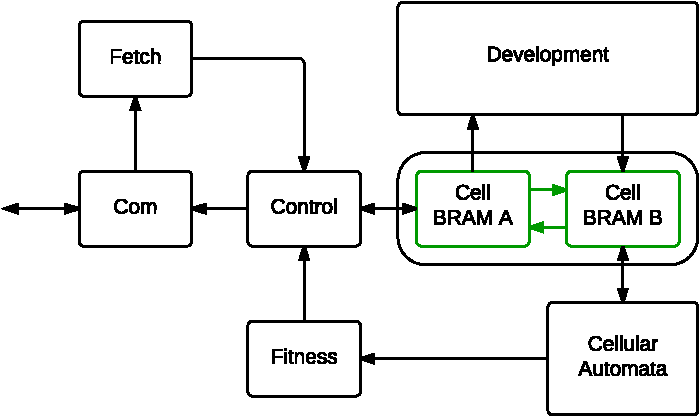
\includegraphics[width=39\block]{implementation-simple}
    \caption[High-level system diagram]{
        High-level block diagram of the new hardware platform.
    }
    \label{fig:implementation-simple}
\end{figure}


The new platform is nearly identical in overall structure to the previous, as shown in \figurename~\ref{fig:implementation-simple},
However, there are a lot of underlying changes to reduce complexity and improve reliability and scaling.
A more detailed view of the system in shown in \figurename~\ref{fig:implementation-full}.

Conseptually, the platform is a three-stage interlocked pipeline with the stages Fetch, Decode and Execute, where the Execute stage includes the Control, Development and CA modules.
Only one module within each stage is activated at a time, and the interlocking allows each module to contain further pipelines without requiring complex hazard detection and evasion.
%At one point there is a pipeline within a pipeline within a pipeline.
Fitness is special in that it is not part of the main pipeline since it operates in a dataflow-like fashion.

\begin{sidewaysfigure}[!pt]
    \centering
    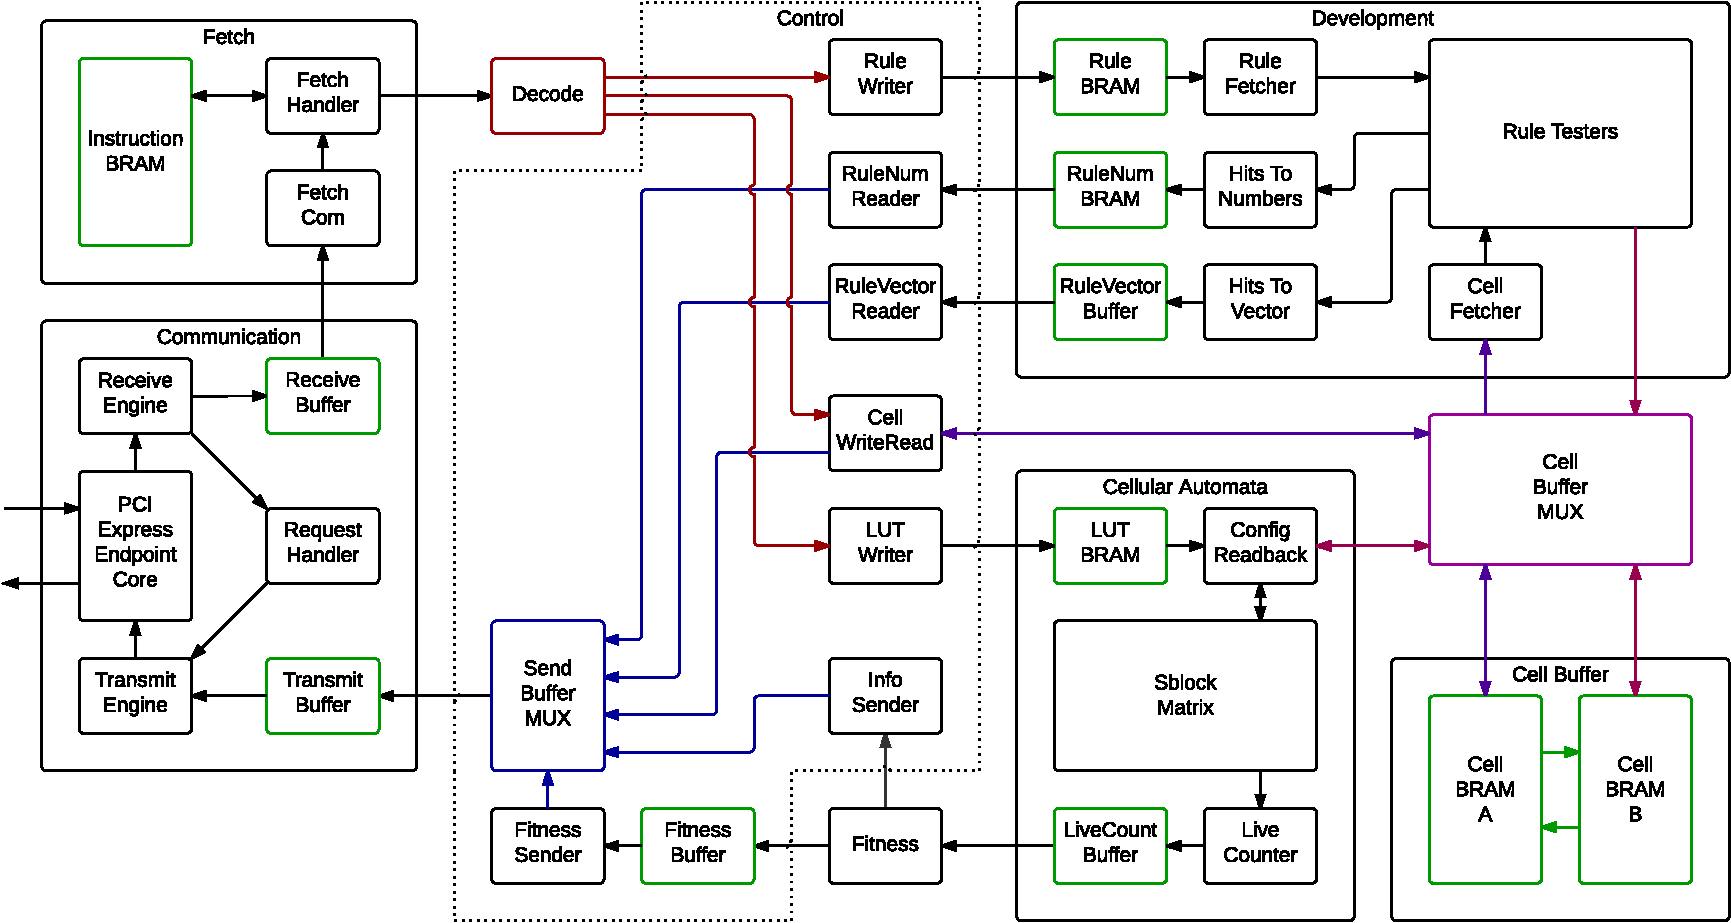
\includegraphics[width=\textwidth]{implementation-full}
    \caption[Detailed system diagram]{
        Detailed block diagram of the new hardware platform.
        Control is implemented as a group of modules, marked by a dotted border.
        Some signals are color-coded for increased readability.
        Signals from Decode are colored red, while those to the Send Buffer and Cell Storage Multiplexers are colored blue and purple respectively.
        Note the two different hues of purple for the different Cell BRAMs.
        Control signals are not shown.
    }
    \label{fig:implementation-full}
\end{sidewaysfigure}

%==============================================================================%

\section{General Concepts}

Some concepts are used repeatedly throughout the design.
The main ones are parameterization, pipelining, buffers and states machines.
The first three are general and are detailed in the following sections.
The state machines vary from module to module and are therefore detailed where appropriate, but all are of Mealy design with clocked output.

\subsection{Parameterization}

Almost every part of the design is parameterized, usually with little restriction on the range of values.
Where restrictions do apply, asserts have been placed in the code of the modules that do restrict them.
These alert the user of correct values during synthesis, and pinpoints the code that must be changed in the event of an expansion.
Keep in mind though that the ISA must likely be changed as well.
The list of parameters is shown in Table~\ref{tab:parameters}.

\begin{table}[!ht]
    \renewcommand{\arraystretch}{1.3}
    \centering
    \begin{tabular}{l|c|l}
        \bfseries Parameter & \bfseries Values & \bfseries Notes \\
        \hline
        Communication Buffer Size Lg & [$1,\infty$] & $log_2$ of buffer size \\
        Communication Reverse Endian & $True,False$ & Required for x86 systems \\
        Program Counter Bits         & [$1,16$]     & Restricted by ISA/Decode \\
        Matrix Width                 & [$2,256$]    & Restricted by ISA/Decode \\
        Matrix Height                & [$2,256$]    & Restricted by ISA/Decode \\
        Matrix Depth                 & [$1,256$]    & Restricted by ISA/Decode \\
        Matrix Wrap                  & $True,False$ & \\
        Type Bits                    & [$1,32$]     & Restricted by ISA/Decode \\
        State Bits                   & $1$          & Restricted by Sblocks \\
        Counter Amount               & [$1,256$]    & Restricted by ISA/Fetch \\
        Counter Bits                 & [$1,32$]     & Restricted by ISA/Fetch \\
        LUT Configuration Bits       & $1,2,4,8$    & Restricted by Sblocks \\
        Rule Amount                  & [$1,\infty$] & \\
        Rules Tested In Parallel     & [$1,\infty$] & \\
        Rule Vector Buffer Size      & [$1,\infty$] & \\
        Fitness Buffer Size          & [$1,\infty$] & \\
        Fitness Module Name          & $Special$    & Without ``fitness\_'' prefix \\
    \end{tabular}
    \caption[Parameters.]{Parameters with supported values.}
    \label{tab:parameters}
\end{table}

\subsection{Pipelining}

The new hardware design makes extensive use of pipelining, and since many stages use a variable amount of cycles for a variety of reasons, interlocking is used in nearly all pipelines.
Interlocking is implemented with two signals connected to each stage: Run and Done.
When a stage does not require further cycles to finish, it asserts its Done signal and then waits for the Run signal before continuing.
The Run signals for all stages are asserted when all Done signals are asserted.
Each stage then resets its Done signal and the process repeats.
An example is shown in \figurename~\ref{fig:wavediagram-pipeline}.

\begin{figure}[!ht]
    \centering
    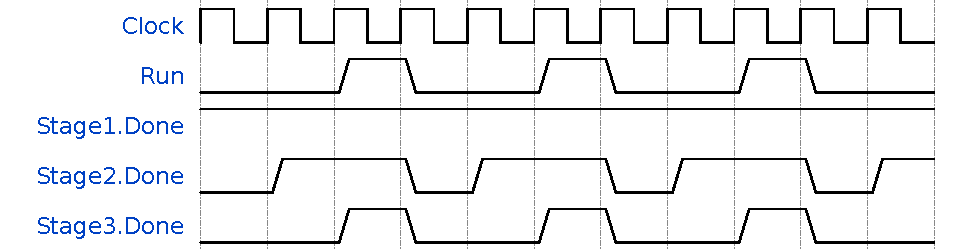
\includegraphics[width=0.86\textwidth]{wavediagram-pipeline}
    \caption[Pipeline wave diagram]{
        Wave diagram showing pipeline interlocking signals for a 3-stage pipeline where the stages complete in one, two and three cycles respectively.
    }
    \label{fig:wavediagram-pipeline}
\end{figure}

Often, a multi-cycle stage only looks at its input in the first cycle to determine its execution path.
This can be taken advantage of to reduce register usage by ruling that the data in the pipeline registers only have to be valid when Run is asserted.
The stages can then write directly to their output registers, instead of caching partial output internally in extra registers.
If a stage happens to require the output of the previous stage for multiple cycles however, input caching is needed.
This causes no register usage reduction in the worst case, while the register usage is halved in the best case.
The common case for this design is to only look at the input the first cycle for most signals, which should provide a nice reduction.

\subsection{Buffers}

All buffers are implemented as first-in first-out (FIFO) queues using block RAM (BRAM) and two counters.
The counters determine the addresses that are written to and read from, and are incremented when the write or read signals are asserted.
\figurename~\ref{fig:wavediagram-fifo} shows how the FIFO is used to buffer two words.

\begin{figure}[!ht]
    \centering
    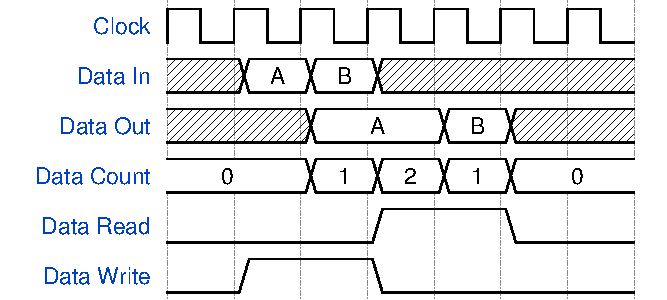
\includegraphics[width=0.64\textwidth]{figures/wavediagram-fifo}
    \caption[FIFO buffer wave diagram]{
        Wave diagram for the FIFO buffer, showing two consecutive writes followed by two consecutive reads.
    }
    \label{fig:wavediagram-fifo}
\end{figure}

Notice how the read signal needs to be asserted before the clock tick when data is read to ensure correct consecutive reads.
This is due to the BRAM used in the FIFO, which updates at clock ticks.
To have correct data available for a read in the following cycle, the address therefore has to be updated before the clock tick (by asserting the read signal).

%==============================================================================%

\section{Communication}

The new communication unit is based on Xilinx' reference PCI Express programmed input/output design.
It consists of the Xilinx PCI Express endpoint core, reception and transmission engines, data buffers, and a special request handler, as shown in \figurename~\ref{fig:implementation-communication}.

\begin{figure}[!ht]
    \centering
    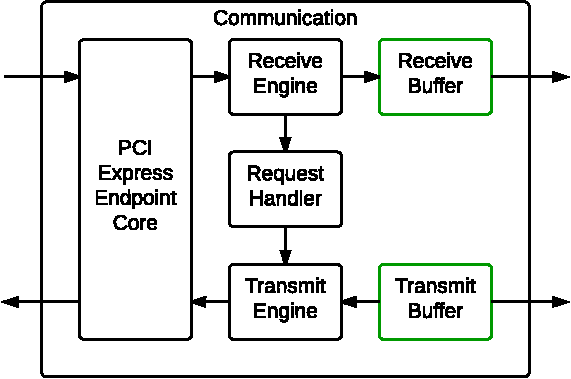
\includegraphics[width=36\block]{implementation-communication}
    \caption[Communication module]{
        Detailed block diagram of the communication module.
    }
    \label{fig:implementation-communication}
\end{figure}

The endpoint core completely handles the physical and data link layers, and all TLPs related to configuration and establishment of the PCI Express connection.
The reception engine is responsible for parsing TLPs and either writing received data to the reception buffer or notifying the transmission engine about a read request.
The transmission engine is responsible for building completer TLPs to respond to read requests, using data from the transmission buffer.
The request handler listens to the read requests provided by the reception engine, and can override the transmission engine to respond to special requests.

\subsection{PCI Express Endpoint Core}

Several Spartan-6 FPGAs, including the one used in this project, contain a special-purpose hardware block for implementation of PCI Express.
The block completely handles the physical and data link layers, with the transaction layer left for the user.

To make use of the block, Xilinx provides the Spartan-6 Integrated PCI Express Endpoint Core; version 2.3 was used in this project.
This core additionally takes care of all TLPs related to configuration of the PCI Express connection.
Other TLPs, such as read and write requests, are presented on an AXI4-Stream interface \cite{ug672}.

The endpoint core is configured with two memory regions, both 4 kB in size\footnotemark.
\footnotetext{
    The smallest memory region that can be memory-mapped is one page. The default page size in Linux is 4 kB.
}
The first memory region (BAR0) is used for normal communication, while the second (BAR1) is used for special requests.
The separation is mostly conceptual as both regions are treated as one data stream.
The difference is that the special request handler kicks in for read requests to BAR1.

\subsection{Reception engine}

The reception engine is implemented as a simple state machine, as shown in \figurename~\ref{fig:statemachine-receive}.

\begin{figure}[!ht]
    \centering
    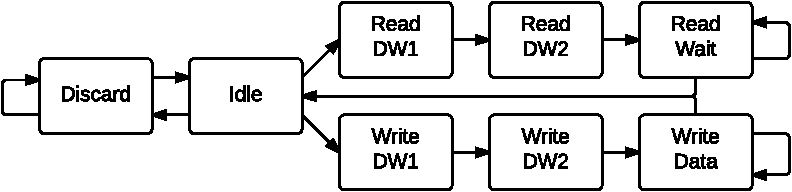
\includegraphics[width=42\block]{statemachine-receive}
    \caption[Reception engine state machine]{
        State machine for the reception engine.
    }
    \label{fig:statemachine-receive}
\end{figure}

Until the endpoint core presents valid data, the state machine remains in Idle.
When it does, the data is stored, and the TLP type is checked.
If it is a read or write request, the state machine continues down the corresponding path, otherwise the remaining data is discarded.
The remaining portion of the TLP headers are then parsed in the DW1 and DW2 states.
For read requests, the state machine waits in ReadWait until the transmission engine is ready to accept a new read request, and then proceeds to Idle.
For write requests, the state machine stays in WriteData, where one DW of data is written to the reception buffer each cycle, for the length of the packet, and then proceeds to Idle.

\subsection{Transmission engine}

The transmission engine is implemented as a simple state machine, as shown in \figurename~\ref{fig:statemachine-transmit}.

\begin{figure}[!ht]
    \centering
    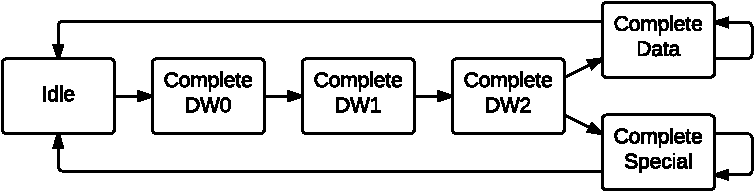
\includegraphics[width=40\block]{statemachine-transmit}
    \caption[Transmission engine state machine]{
        State machine for the transmission engine.
    }
    \label{fig:statemachine-transmit}
\end{figure}

Until the reception engine signals a read request, the state machine remains in Idle.
When a read request is signaled by the reception engine, the state machine begins to traverse the DW path.
The DW0, DW1 and DW2 states each transmit one DW of the completer TLP header.
Then if the special request signal is set, it proceeds to CompleteSpecial, where it transmits data presented by the request handler.
Otherwise, it proceeds to CompleteData where it transmits one DW of data from the transmission buffer each cycle.
When the requested number of DWs has been transmitted it proceeds back to Idle.

\subsection{Request handler}

The request handler continually listens to the read requests presented by the reception engine.
If the request is targeting the primary memory area (BAR 0), it is a normal read request and the transmission engine is allowed to proceed as usual.
Otherwise, it is a special request and the transmission engine is overridden.

The kind of special request is determined by the address of the read request, and handled thereafter.
There are currently four special requests implemented, as shown in Table~\ref{tab:requests}.

\begin{table}[!ht]
    \renewcommand{\arraystretch}{1.3}
    \centering
    \begin{tabular}{c|l}
        \bfseries Address & \bfseries Request \\
        \hline
        0x00 & Get transmission buffer data count \\
        0x01 & Get transmission buffer available space \\
        0x02 & Get reception buffer data count \\
        0x03 & Get reception buffer available space \\
    \end{tabular}
    \caption{Special requests.}
    \label{tab:requests}
\end{table}

Note that each of the implemented special requests assumes a read request length of one DW.
If the request has a greater length, the returned data is simply repeated to fill the packet.

%==============================================================================%

\section{Fetch}

The Fetch module is responsible for retrieving the next instruction that should be decoded and then executed.
It also handles all control flow.
It is implemented as a two-stage interlocked pipeline consisting of a Fetch Communication module and a Fetch Handler module connected to an Instruction BRAM.
This is shown in \figurename~\ref{fig:implementation-fetch}.

\begin{figure}[!ht]
    \centering
    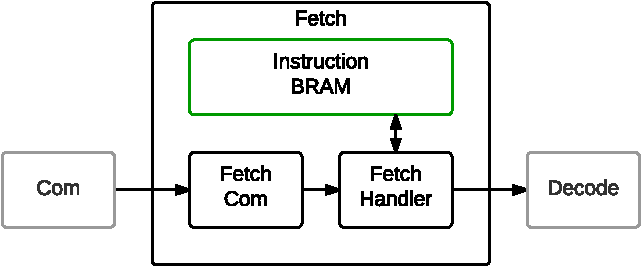
\includegraphics[width=34\block]{implementation-fetch}
    \caption[Fetch module]{Detailed block diagram of the Fetch module.}
    \label{fig:implementation-fetch}
\end{figure}

Fetch Communication is responsible for converting data from the communication module into instructions while the Fetch Handler takes care of control flow and the instruction memory.
Both stages are implemented as state machines, making interlocking necessary.

\subsection{Fetch Communication}

While instructions are 256-bit, the communication interface is only 32-bit.
This means that the host system has to split each instruction into multiple 32-bit pieces.
As detailed in Appendix~\ref{app:isa}, many instructions make use of less than 256 bits.
In fact, most instructions fit within the first 32 bits.
Sending all 256 bits for each instruction is therefore a bit excessive.
To optimize communication, the first 32-bit piece of each instruction has a field declaring the amount of following pieces required for reassembly.

The job of the Fetch Communication module is to combine all the pieces back into full 256-bit instructions.
It starts by reading the first 32-bit piece and setting all other bits to zero.
Then, the 3-bit instruction length field is analysed to determine how many further pieces are part of the same instruction.
The remaining pieces are then incorporated into the instruction, before it is passed on to the Fetch Handler.

\subsection{Fetch Handler}

The Fetch Handler has three modes of operation: FetchCom, FetchMem and StoreMem.
The modes and transitions are implemented as a state machine, which is shown in \figurename~\ref{fig:statemachine-fetch-handler}.

\begin{figure}[!ht]
    \centering
    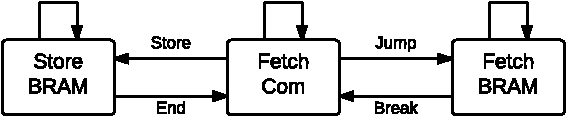
\includegraphics[width=30\block]{statemachine-fetch-handler}
    \caption[Fetch Handler state machine]{State machine for the Fetch Handler.}
    \label{fig:statemachine-fetch-handler}
\end{figure}

In FetchCom mode, instructions are fetched from communication and sent to decode.
Since a variable-length format is used, this may take multiple cycles.
To make sure that instructions does not get ``stuck'' in the pipeline due to no further instructions arriving at the communication interface, NOPs are sent when Fetch Communication is busy.
When encountering a Store instruction, it enters StoreMem mode and for a Jump instructions it enters FetchMem mode.

In FetchMem mode, instructions are fetched from InstructionBRAM and sent to decode.
The first InstructionBRAM address is specified by the Jump instruction, and then it is incremented by one after each instruction.
When encountering a Break instruction, it enters FetchCom mode.
As a safety precaution to prevent lock-ups, FetchCom mode is also entered if the program counter overflows.

In StoreMem mode, instructions are fetched from communication and stored in InstructionBRAM.
The first InstructionBRAM address is specified by the Store instruction, and then it is incremented by one after each instruction.
Instructions are stored in full 256-bit format.
When encountering an End instruction, it enters FetchCom mode.

Control flow is implemented by having N M-bit general counters and a JumpEqual instruction.
The counters can be incremented or reset using special instructions.
The JumpEqual instruction is treated as a Jump instruction when the specified counter matches the specified value, otherwise it is discarded.

%==============================================================================%

\section{Decode}

Decode is responsible for parsing instructions, setting up control signals and passing instruction parameters to activated modules.
It is a very simple module, being essentially a giant switch statement with a case for each instruction.

Control signals are sent to all top-level modules except communication and fetch which operate earlier in the pipeline, and fitness which operates in a dataflow-like manner.
By default, all modules are given a no-operation signal and multiplexers stay unchanged.
Then, depending on the instruction's operation code, the control signal for the appropriate module is set, parameters (if any) are extracted and passed on to the module, and multiplexers are changed if needed.

Each instruction will cause exactly one module to be activated in the Execute stage.
This is to keep the design clean and reduce inter-module dependencies.

%==============================================================================%

\section{Control}

Control is a group of modules, shown in \figurename~\ref{fig:implementation-control}.
Together, the modules control all inputs and outputs for the Cell Storage, CA and Development modules.
Each module is designed to do one specific task and be independent of any other modules.
This means that modules are mostly very simple and that it requires a low amount of effort to add new modules or to modify existing.

\begin{figure}[!ht]
    \centering
    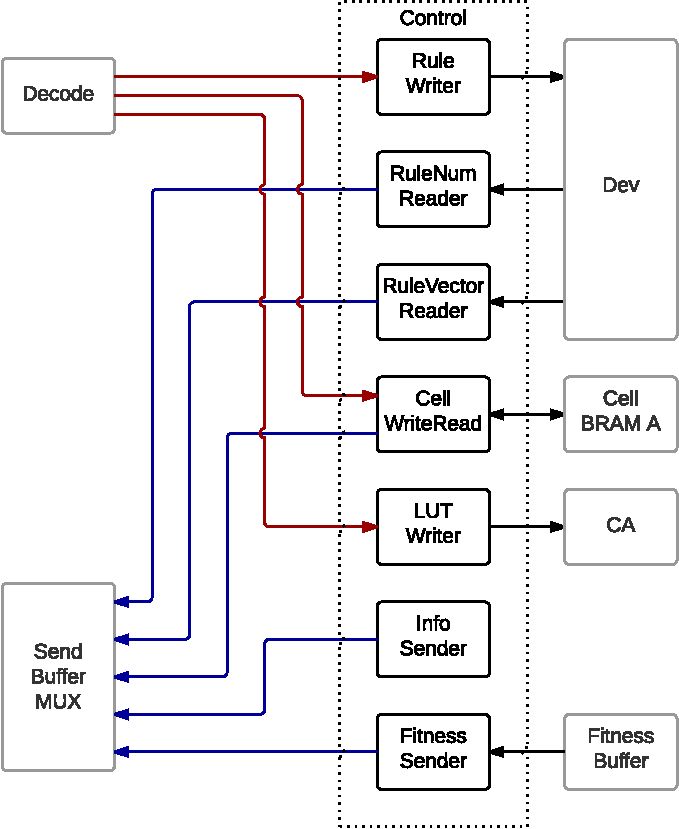
\includegraphics[width=36\block]{implementation-control}
    \caption[Control modules]{
        Detailed block diagram of the Control modules.
        Red signals are inputs while blue are outputs.
        Control signals are not shown.
    }
    \label{fig:implementation-control}
\end{figure}

Following are detailed descriptions of the different modules, in order of increasing complexity.

\subsection{Rule Writer}

The purpose of the Rule Writer is to store new rules to the Rule BRAM within the Development module.
It is, along with the LUT Writer, the simplest control module.
When activated, it stores one rule to a specified index of the Rule BRAM.
The index doubles as priority for a rule, with higher indexes having higher priority.

As explained in Section~\ref{sec:development}, index zero is reserved for representing that no rules have triggered.
Writing a rule to it has no effect as the rule testers are reset instead of testing the rule during development.

\subsection{LUT Writer}

The purpose of the LUT Writer is to store new LUTs to the LUT BRAM within the CA module.
It is, along with the Rule Writer, the simplest control module.
When activated, it stores one LUT to a specified index of the LUT BRAM.
The index is equivalent to the cell type that should be given that LUT during CA configuration.

\subsection{Information Sender}

Nearly all parts of the system are parameterized.
The previous practice of manually ensuring that the parameters of both the design and API were in sync was both tiresome and prone to error.
Therefore, the Information Sender provides a means for the API to automatically query these parameters.

When activated, it puts all parameters that might be useful into the Transmission Buffer.
This includes information about the CA such as the size, whether wrapping is enabled, and number of bits per state and type;
information about counters available for control flow;
maximum number of rules;
and information about the fitness modules, such as the type and output size.

\subsection{Fitness Sender}

The Fitness Sender is responsible for sending the output of the Fitness module to the host.
This is a simple matter of moving data from the Fitness Buffer to the Transmission Buffer when data is available in the first and there is space in the second.
The number of words that is transferred per activation is declared by the Fitness module (see Section~\ref{sec:fitness}).
Keep in mind that the machine will go into a deadlock if insufficient data is produced for the Fitness buffer.

\subsection{Rule Vector Reader}

The Rule Vector Reader is tasked with reading one or more rule vectors created by the Development module and sending them to the host.
Since rule vectors can be of any length, they are each split over multiple words, starting with the lowest indexes.
The final word of each vector is padded with zeroes.
For more information on rule vectors, see Section~\ref{sec:development}.
Keep in mind that the machine will go into a deadlock if insufficient data is produced for the Rule Vector buffer.

\subsection{Rule Numbers Reader}
\label{sec:rule-numbers-reader}

The Rule Numbers Reader is tasked with reading each cell's most recently activated development rule and sending them to the host.
The rule numbers are stored in the Rule Numbers BRAM of the Development module and are scanned in raster order\footnotemark.
Each word is fitted with as many rule numbers as possible without splitting them over multiple words or containing ones from different rows.
Any remaining space is filled with zeroes.

\footnotetext{
    In raster scanning, two-dimensional data is read line-by-line, least significant to most significant.
    This is extendable to 3D; increment X first, then Y, then Z.
}

\subsection{Cell Writer Reader}

The purpose of the Cell Writer Reader is to perform read and write operations against Cell BRAM A, causing it to be the system's main input/output channel.
It is possible to write states and types to either a single cell, a row of cells or the entire BRAM, while it it is possible to read from a single cell or the entire BRAM.

It is easily the most complex control module, due to the intricate operations required to change only selected values in BRAM rows.
Additionally, it must convert variable-width types and states into fixed-width words in an efficient manner when reading.

The module consists of combiners which are used to combine new data with existing data from the Cell BRAM, repeaters to simplify the process of filling the entire Cell BRAM with a given state and type, shifters used to select output, and a state machine which controls everything.
\figurename~\ref{fig:implementation-cell-writer-reader} shows how the components are connected.

\begin{figure}[!ht]
    \hspace{-1\block}
    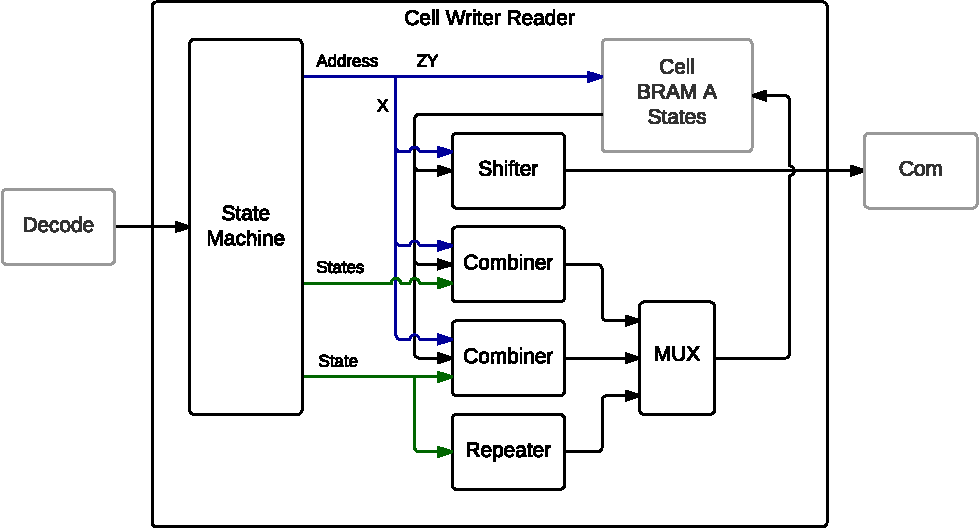
\includegraphics[width=52\block]{implementation-cell-writer-reader}
    \caption[Cell Writer Reader]{
        Detailed block diagram of the Cell Writer Reader.
        Only the state part is shown to reduce complexity; the type part is identical.
        Cell BRAM A is drawn inside the module for completeness.
        Control signals are not shown.
    }
    \label{fig:implementation-cell-writer-reader}
\end{figure}

\subsubsection{Combiner}

The combiner is a combinatorial unit that combines two signals of different lengths by replacing one part of the long signal with the short signal.
This is implemented using a shifter and a mask that is the size of the short signal.
First, the short input and mask is shifted into the desired position.
Then, the long signal is AND-ed with the inverted mask and OR-ed with the short signal, producing the combined signal.
The process is illustrated in \figurename~\ref{fig:combiner}.

\begin{figure}[!ht]
    \centering
    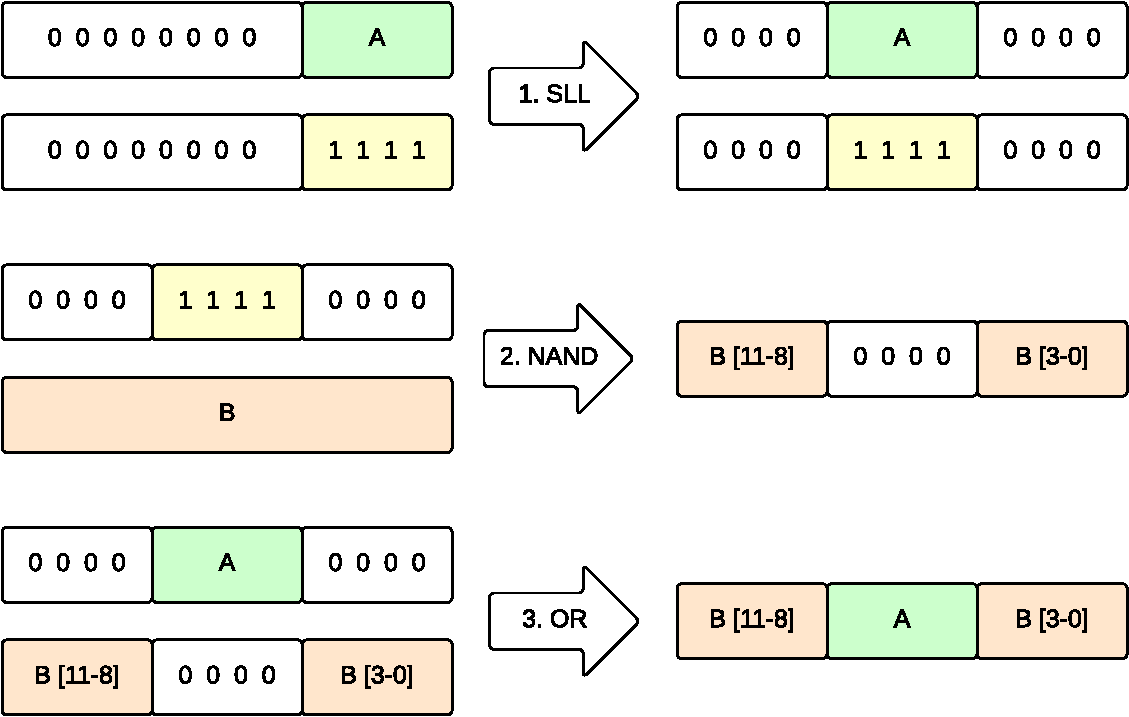
\includegraphics[width=0.8\textwidth]{combiner}
    \caption[Combiner operation]{
        The three operations that power the combiner.
        A is the short input, highlighted in green.
        B is the long input, highlighted in orange.
        The mask is highlighted in yellow.
    }
    \label{fig:combiner}
\end{figure}

\subsubsection{State Machine}

The state machine consists of seven states, shown in \figurename~\ref{fig:statemachine-cell-writer-reader}.
When an operation is received, the BRAM address is set and it transitions from idle to the corresponding state.
Some states are dual-purpose due to the similarity of the operations, while others are not.
Coincidentally, the dual-purpose states complete in one cycle while the others require multiple\footnotemark.
\footnotetext{
    Technically, the Send One state does not necessarily complete in one cycle since it will wait until there is available space in the Transmission Buffer.
    However, it is the common case.
}

\begin{figure}[!ht]
    \centering
    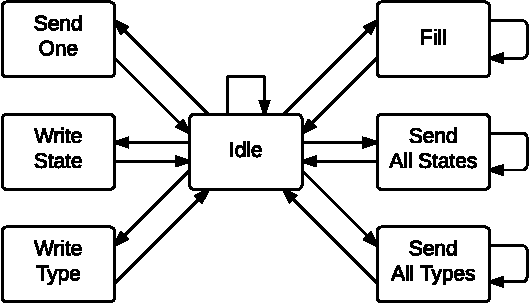
\includegraphics[width=28\block]{statemachine-cell-writer-reader}
    \caption{Cell Writer Reader state machine}
    \label{fig:statemachine-cell-writer-reader}
\end{figure}

The dual-purpose states are as follows:
Send One can send either a state or a type, Write State can write either one or a row of states, and Write Type can write either one or a row of types.
The remaining states are:
Fill writes the same state and type to all cells, Send All States reads all states in raster order, and Send All Types reads all types in raster order.
The output formatting of the Send All states is equal to that of the Rule Numbers Reader, detailed in Section~\ref{sec:rule-numbers-reader}.

%==============================================================================%

\section{Cell Storage}

The Cell Storage serves as the location for exchange of cell data between the CA, Development and Host.
It contains two separate storage areas, the contents of which can be swapped.
Each storage area can host a full matrix of cell states and types, and allows one row of each to be read each cycle.
The main reason two storage areas are needed is the Development module.
It requires a place to store its output without affecting its input during the development process.
More on this in Section~\ref{sec:development}.

The module is implemented as two dual-port BRAMs, one for states and one for types, each sized to twice the size of the matrix.
To create two separate storage areas (A and B) with both states and types, the address of the first port is prefixed with 0 and the second with 1.
The contents of the storage areas can then be made to appear swapped by simply inverting the prefix bits.

To service all required components, the Cell Storage is connected via a multiplexer.
It has two modes; normal and development.
In normal mode, storage A is connected to the Cell Writer Reader and storage B to the CA.
In development mode, both storage areas are connected to the Development module.

\todo{fig?}

%==============================================================================%

\section{Development}
\label{sec:development}

The Development Module is responsible for providing the ontogenetic aspect of the system by allowing cells to be changed based on user-supplied development rules described in Appendix~\ref{app:isa}.
It uses Cell Storage A as input and outputs the modified cells to Cell Storage B.

The module is implemented as a two-stage interlocked pipeline controlled by a state machine.
Stage one contains the Cell Fetcher, which retrieves cell neighborhoods from Cell BRAM A, and stage two contains a four-stage pipeline that tests development rules against the cell neighborhoods.
This is illustrated in \figurename~\ref{fig:implementation-development}.

\begin{figure}[!ht]
    \hspace{-4\block}
    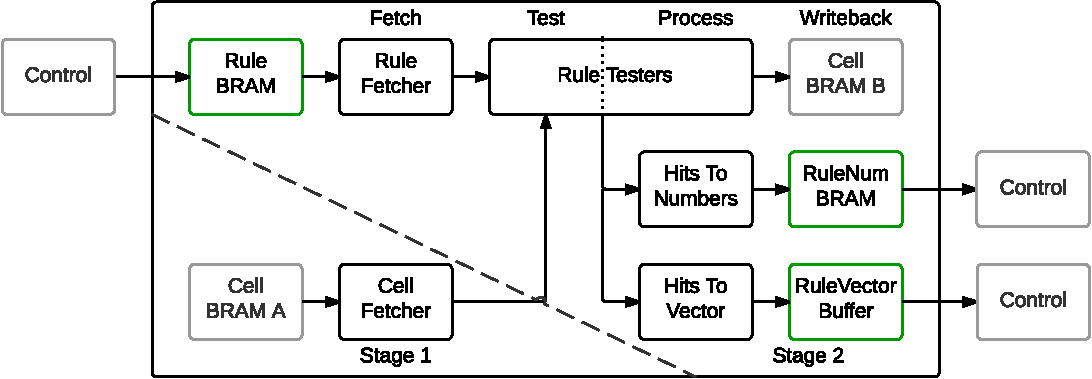
\includegraphics[width=58\block]{implementation-development}
    \caption[Development module]{
        Detailed block diagram of the Development module.
        The two main pipeline stages are separated by a dashed line,
        while the sub-stages of the pipeline within the second main stage are marked at the top.
        The cell BRAMs are drawn inside the module for pipeline completeness.
        Control signals are not shown.
    }
    \label{fig:implementation-development}
\end{figure}

The state machine, shown in \figurename~\ref{fig:statemachine-development}, ensures proper timing of the complex pipeline.
It is responsible for setting input and output addresses, activating pipeline stages and setting write signals.
A complete timing diagram can be seen in \figurename~\ref{fig:wavediagram-development}.

\begin{figure}[!ht]
    \centering
    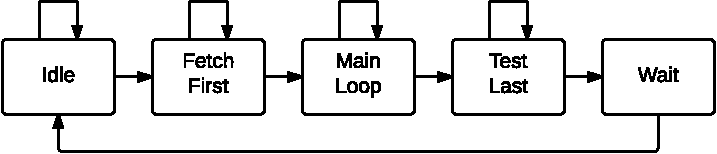
\includegraphics[width=38\block]{statemachine-development}
    \caption[Development module state machine]{
        State machine controlling the Development module.
    }
    \label{fig:statemachine-development}
\end{figure}

\begin{sidewaysfigure}[!pt]
    \centering
    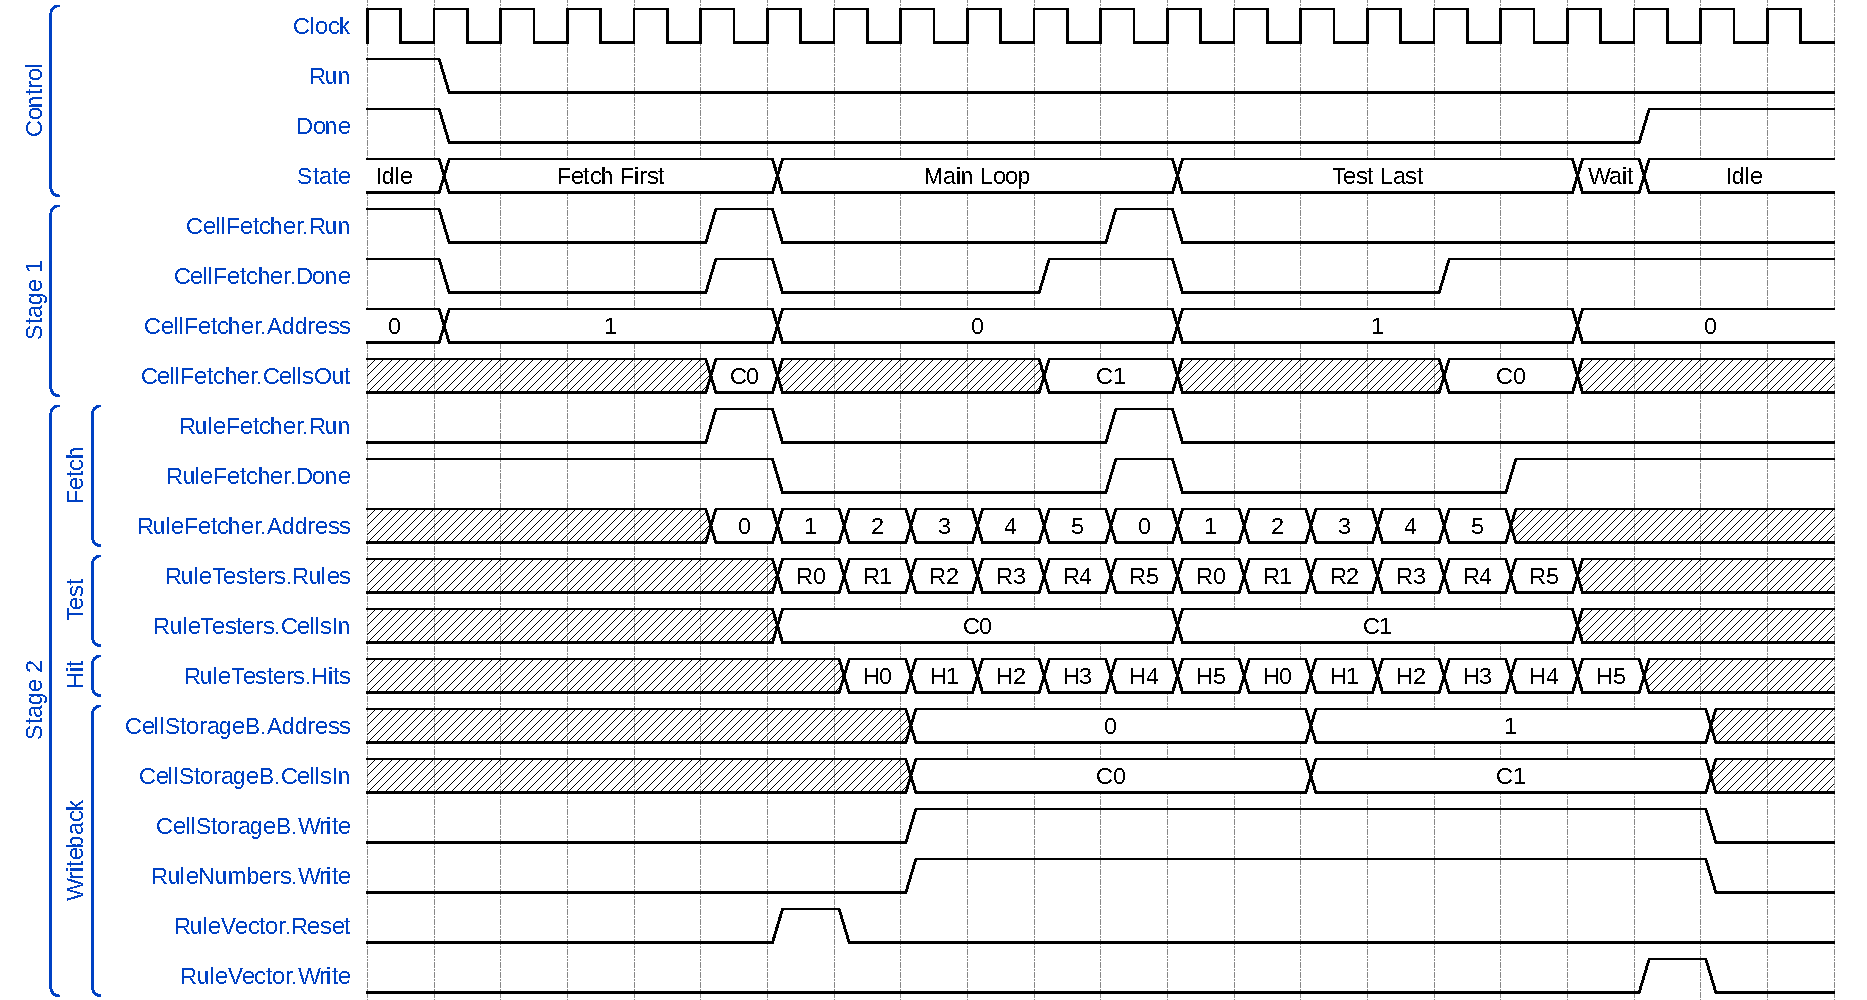
\includegraphics[width=\textwidth]{wavediagram-development}
    \caption[Development module wave diagram]{
        Wave diagram for the Development module, showing the development process for an Nx2 matrix with five active rules.
    }
    \label{fig:wavediagram-development}
\end{sidewaysfigure}

\subsection{Cell Fetcher}

The Cell Fetch reads the cell neighborhoods for one row of cells from Cell BRAM A per run.
It is implemented as two state machines, one which sets the BRAM address and one which retrieves the output.
The first can be seen in \figurename~\ref{fig:statemachine-cell-fetcher}.
The other is equivalent to the first except for being delayed two states, thus having Wait 1 as initial state instead of Fetch Center.

\begin{figure}[!ht]
    \centering
    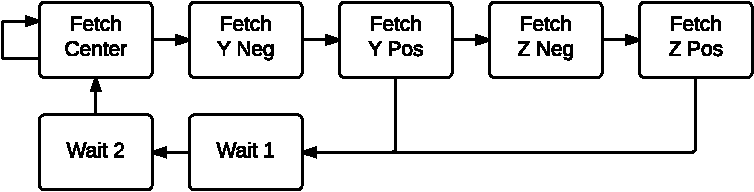
\includegraphics[width=40\block]{statemachine-cell-fetcher}
    \caption[Cell Fetcher state machine]{
        State machine for the Cell Fetcher.
    }
    \label{fig:statemachine-cell-fetcher}
\end{figure}

By reading an entire row at a time, the neighbors along the X axis are fetched ``for free'', while the other axes require two extra reads each.
This lands the runtime on 5 cycles for 2D matrices and 7 cycles for 3D when including BRAM latency.
The Cell Fetcher is therefore only a limiting factor when there are very few active rules.

By default, neighbors which would be outside the matrix are treated as having zero for both state and type.
However, it is possible to enable matrix wrapping to instead use the neighbors on the opposite side of the matrix.

\subsection{Rule Fetcher}

The Rule Fetcher is responsible for fetching development rules from Rule BRAM and passing them to the Rule Testers.
It takes into account the specified number of active rules to speed up the development process by only fetching those.
It is possible to further improve performance by setting that multiple rules should be fetched and tested at the same time.
In that case, those with indexes higher than the number of active rules within the last rule batch are replaced by rules with no effect.

\subsection{Rule Testers}

The Rule Testers are responsible for testing development rules received from the Rule Fetcher against cell neighborhoods received from the Cell Fetcher.
They are unique in that they produce output after both one and two cycles.
Information about rule activations, ``hits'', are passed on to the hit processors after one cycle, and the result of the rule application is passed on to Cell BRAM B after two cycles.
Rule hits undo any effects of previous hits so that it is impossible for two rules to have simultaneous partial effects, in cases where one modifies only the state and the other only the type.

There is a special case for rule zero.
It is used as an internal reset by forcing a hit and setting the output cell to the input cell.
This implementation was chosen because of its simplicity and the ability to use zero to mean ``unchanged'' in the hit processors.
It also makes it possible to have no active rules.

\subsection{Hit Processors}

There are two modules dedicated to providing information about the development procedure, Hits To Vector and Hits To Numbers.
The input for both are hits passed on from the Rule Testers.

Hits To Vector stores a vector where each bit signifies whether the rule of that index was triggered or not to the Rule Vector Buffer after each development phase.
Rules that have triggered but is later overridden by a rule with higher priority is still marked as having been triggered in the vector.
If the buffer is full, it is reset instead of waiting, to allow programs to disregard the data without causing deadlocks.

Hits To Numbers stores the index of the last triggered rule for each cell to the Rule Numbers BRAM.
Since rule zero is always marked as a hit, the BRAM is reset to zeroes at the beginning of each development phase, and then overwritten by before the rule numbers are written.

%==============================================================================%

\section{Cellular Automata}

The CA module is the centerpiece of the system.
It is what contains the sblock matrix and the control logic to service it.
The module is responsible for configuring the sblock matrix with data from Cell BRAM B, step the sblocks and store the number of live cells afterwards, and write the new states back to Cell BRAM B.

The implementation can be seen in \figurename~\ref{fig:implementation-cellular-automata}.
It consists of a state machine, the Sblock Matrix and a Live Counter, in addition to storage for LUTs and a buffer for the Live Counter.

\begin{figure}[!ht]
    \centering
    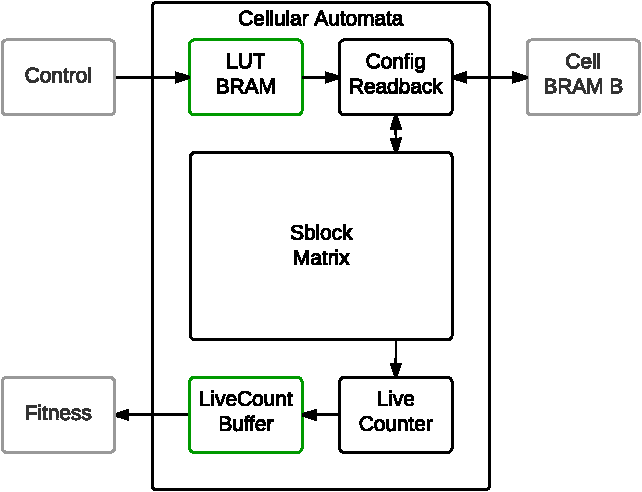
\includegraphics[width=34\block]{implementation-cellular-automata}
    \caption[CA module]{
        Detailed block diagram of the CA module.
        Config Readback is a symbolic module for the majority of the state machine.
    }
    \label{fig:implementation-cellular-automata}
\end{figure}

\subsection{State Machine}

The state machine in \figurename~\ref{fig:statemachine-cellular-automata} is what powers this module.
It is what controls both configuration, readback and stepping of the Sblock Matrix.
Additionally, it sets write signals for the Live Count buffer.

\begin{figure}[!ht]
    \centering
    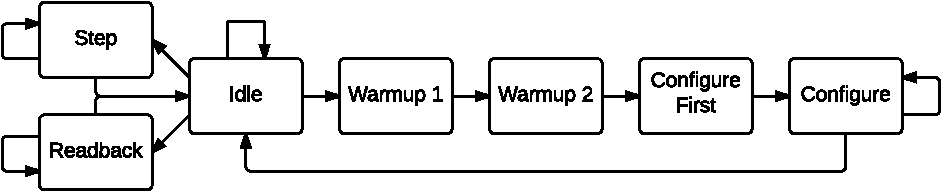
\includegraphics[width=50\block]{statemachine-cellular-automata}
    \caption[CA module state machine]{
        State machine controlling the CA module.
    }
    \label{fig:statemachine-cellular-automata}
\end{figure}

Configuration is the process of taking cells from Cell BRAM B, converting them into LUTs and programming the sblocks.
It operates on one row of cells/sblocks at a time.
First, the cells are read from Cell BRAM B and the type of each are used as addresses for the 1-in N-out LUT BRAM to find the corresponding LUT.
The LUTs are then loaded into shift registers and transfered to the sblocks piece by piece.
Finally, the outputs of the sblocks are set to the states of the cells.

Readback is the process of extracting the cell states from the Sblock Matrix and storing them back in Cell BRAM B.
This operation also works on one row at a time.
However, it is much simpler and faster than configuration since it simply directs the output of the sblocks to the Cell BRAM and sets the correct row.

Stepping is simply the process of telling the Sblock Matrix to update the state of each of its sblocks.
The new state is determined by the using the neighbor states as the input to the LUT, according to the format detailed in Appendix~\ref{app:isa}.
Since it is common to step hundreds of times in a row, the step instruction has a parameter for the number of steps, up to a maximum of 65535 (a 16-bit number).

\subsection{Sblock Matrix}

The Sblock Matrix essentially contains enormous amounts of sblock as they are described in Section~\ref{sec:sblock}.
The only difference is that the sblocks used here have support for configuring multiple bits of the LUT each cycle.
However, to use the dedicated shift registers as configurable LUTs, there are some restrictions on the number of bits.
Firstly, it can only be powers of two; secondly, it can be maximum 2 for 2D matrices and 8 for 3D.
Keep in mind that each bit adds one extra signal for each sblock, which accumulates to a significant amount of routing resources.

By default, neighbors which would be outside the matrix are treated as having zero for both state and type.
However, it is possible to enable matrix wrapping to instead use the neighbors on the opposite side of the matrix.
This option lets the user decide if programs should be able to exploit the matrix size when for example creating oscillators.

\subsection{Live Counter}

The Live Counter is essentially a giant adder tree that is connected to the output of each sblock.
It calculates the total number of live cells after each CA step and stores them in the Live Count Buffer.
Due to the massive amount of sblocks, the calculation is spread out over many cycles, the exact number of which is dependant on the number of sblocks.
However, the throughput remains at one total per cycle.

If the Live Count Buffer happens to be full, it is reset instead of waiting, to allow programs to disregard the data without causing deadlocks.
This will likely corrupt all fitness evaluation until the buffers are reset however.

%==============================================================================%

\section{Fitness}
\label{sec:fitness}

The Fitness module is responsible for evaluating the output of the CA for use with evolutionary algorithms.
Since fitness evaluation vary widely between applications, the interface of the Fitness module is designed to be simple and generic, such that the module is easy to replace.

It is connected in a dataflow-like manner between the Live Count Buffer and the Fitness Buffer.
Whenever there is enough data available in the Live Count Buffer, it should fetch that data, processes it, and store the result to the Fitness Buffer.
The host can then later retrieve it by activating the Fitness Sender.

To comply with the adaptive interface, there are a few things that the Fitness module needs to tell the other parts of the system.
First is the number of words per result, required by the Fitness Sender.
Second is a unique identifier that is reported to the host by the Information Sender.
To allow further versatility, the module can also report synthesis parameters to the host.

There are currently two implemented fitness modules: Live Count and DFT.

\subsection{Live Count}

The Live Count fitness module is used to transfer the live counts to the host for software-side fitness evaluation.
The implementation is as simple as it gets.
The output of the Live Count Buffer is fed directly into the Fitness buffer, and the write and read signals are activated when the Live Count Buffer has data and the Fitness Buffer has space.

\subsection{DFT}

The DFT fitness module uses a Discrete Fourier Transform to convert the live count data into frequency spectrums.
This has the advantage of being able to pick up certain information that might be near-impossible to detect using conventional means.
As shown in \cite{berg2013ca}, using a DFT to interpret CA output holds potential.

A DFT of transform size N takes N complex numbers as input and produces N complex numbers as output.
For transforms where input numbers are all real, the second half of the output mirrors the first half and can be safely ignored to save computation effort.
Each output value of the DFT is a linear combination of all input values.
The constants, which are known as twiddle factors, rely only on the transform size and can therefore be computed ahead of time to reduce the complexity of the calculations.
\todo{a bit funky, move to background?}

This module is essentially a revised version of Støvneng's design in \cite{stovneng2014sblock}.
It has been refactored, streamlined and adapted to fit into the new design.
It is also more customizable, supporting parameters other than powers of two, and can generate twiddle factors by itself during synthesis instead of relying on an external program.
The twiddle factors are stored in a fixed-point format since they range from $-1$ to $1$, and in the order they are needed.

\begin{figure}[!ht]
    \centering
    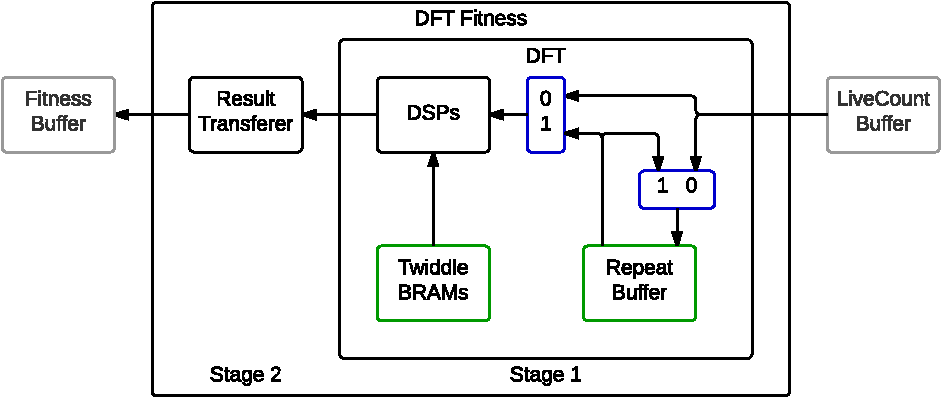
\includegraphics[width=48\block]{implementation-dft}
    \caption[DFT Fitness]{
        Detailed block diagram of the DFT Fitness module.
        The two pipeline stages are marked at the bottom.
        Blue boxes are multiplexers.
        Control signals are not shown.
    }
    \label{fig:implementation-dft}
\end{figure}

To allow the DFT to continue processing while results are transferred from the DFT to the Fitness Buffer, the module is divided into two pipeline stages.
This can be seen in \figurename~\ref{fig:implementation-dft}.
The first stage contains the DFT while the second contains the logic for transferring the result.
The pipeline is interlocked, since both stages can run for hundreds of cycles.

\begin{figure}[!ht]
    \hspace{-1\block}
    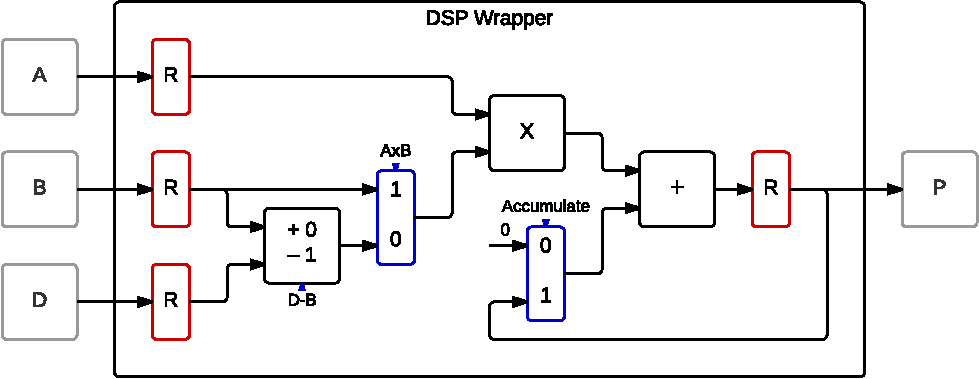
\includegraphics[width=52\block]{implementation-dsp}
    \caption[DSP Wrapper]{
        Detailed block diagram of the DSP Wrapper.
        Red boxes are registers and blue boxes are multiplexers.
    }
    \label{fig:implementation-dsp}
\end{figure}

The DFT is calculated using the DSP slice wrappers seen in \figurename~\ref{fig:implementation-dsp} in multiply-accumulate mode.
Afterwards, the real and imaginary parts of each output value are combined into a single positive number by adding the absolute value of both.
The most optimal configuration would be two DSP slices per output value, one for each real and imaginary part.
However, FPGAs have a limited number of DSP slices.
For larger transform sizes, the DSPs therefore have to calculate multiple output values in sequence.
Since the Live Count Buffer, as all FIFO buffers, is delete-on-read, an internal buffer is used to repeat the values.
This Repeat Buffer is flushed and filled during the first calculation phase and then repeats the values to the DSPs during subsequent phases while also feeding the values back into itself.
The state machine controlling the DFT is shown in \figurename~\ref{fig:statemachine-dft}.

\begin{figure}[!ht]
    \centering
    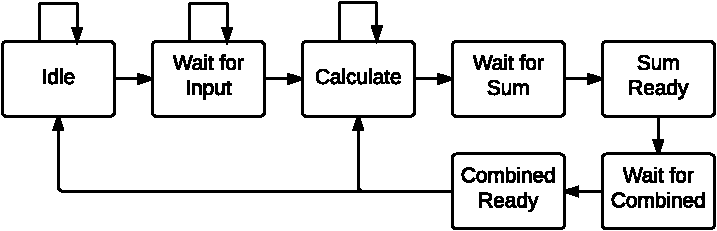
\includegraphics[width=38\block]{statemachine-dft}
    \caption[DFT State Machine]{
        State machine controlling the DFT.
    }
    \label{fig:statemachine-dft}
\end{figure}

%==============================================================================%

\section{Software API}

In accord with the hardware design, the software API has also been given a major overhaul.
Everything has been rewritten from scratch to improve clarity, functionality and ease of use.
\figurename~\ref{fig:api} illustrates the API structure: A main API is used to connect to the hardware platform, send instructions and receive data; and two optional APIs allow conversion of the received data into human-readable forms.

\begin{figure}[!ht]
    \centering
    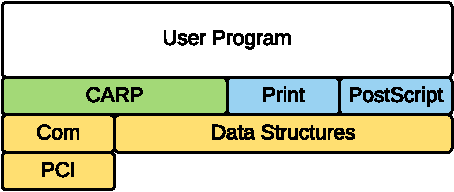
\includegraphics[width=24\block]{api}
    \caption[API]{
        API structure.
        The main API is colored green, optional APIs blue and dependencies yellow.
    }
    \label{fig:api}
\end{figure}

\subsection{Main API}

\TODO

Connect: Clears any remaining data in the buffer, queries synthesis information.
Disconnect: Clears any remaining data in the buffer.
Reset: Everything (\todo{program memory})

All instructions (one function for each). LUTs and development rules are sent as structs.

Getter functions that parse data sent from the FPGA into data structures.

\subsection{Optional APIs}

\TODO

There are two optional APIs, both for converting data structures into output: Print and PostScript.

Print: Information, matrix (states, types and rule numbers), rule vector.

Postscript: Creates postscript image from a matrix (one layer), can supply a coloring function (that returns hex codes).

\subsection{Communication}

The communication part of the new software API is split into two parts:

The first is a general interface for connecting to PCI and PCI Express devices without using a custom driver.
It takes advantage of Linux' automatic population of /sys/devices/pci* with files representing the memory regions of all PCI and PCI Express devices.
The directory is searched by vendor and device id, and the corresponding memory regions are memory-mapped into the program.
Due to this direct interaction with device files, each program must be run with superuser rights.

The second is an interface specifically for the communication unit.
It provides open, close, read and write functions similar to the old BenERA interface, in addition to implementing all special request functions in Table~\ref{tab:requests}.
When a read or write operation is initiated, buffers are checked for available data or space.
If there is not enough present, the program waits and then rechecks.

\subsection{Compilation}

The compilation system has been streamlined to allow users to simply add new files in \textbf{libcarp/} or \textbf{programs/}, and have them automatically be integrated into the API or compiled with the API respectively by calling \textbf{make}.

First, all files in \textbf{libcarp/} is compiled to the statically linked library \textbf{libcarp.a}.
Then each file in \textbf{programs/} is compiled with references to all the header files in \textbf{libcarp/} and \textbf{libcarp.a}.
Programs must include \textbf{carp.h} to use the main API and optionally \textbf{print.h} and \textbf{postscript.h} for the output APIs.

To facilitate unit testing, all programs whose name start with \textbf{test\_} are executed in sequence when \textbf{make test} is called.
\textbf{testframework.cinclude} is provided as a common assertion framework.

\subsection{Compile Parameters}

\TODO

Testbench mode:
Mock info struct with parameters in makefile.
Program exits on buffer flush (triggered when a function that reads data is called).

Low-latency mode:
Recheck buffers immediately instead of waiting for one microsecond.

Debug mode:
Wait 100ms between buffer rechecks and print progress.
Print all data cleared from the buffer.
Notify of reset and clear.


\chapter{Verification}
    \label{ch:verification}
    \TODO

\section{Functionality}

\TODO
Tests use shared framework.
One test program for each instruction approx.

\section{Performance}

\TODO

\section{Fitness}

\TODO

\section{Example}

\todo{make into chapter?}

\begin{itemize}
    \item 21 rules and 13 states.
    \item Green goes in circle to form border, red when complete (but not corners).
    \item Cyan detaches from corners to form new circles.
    \item X increases to the right, Y increases downwards.
\end{itemize}

\begin{figure}[!ht]
    \centering
    \begin{subfigure}{0.32\textwidth}
        \centering
        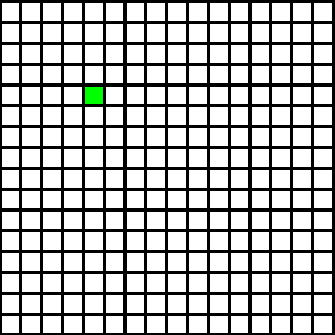
\includegraphics[width=0.9\textwidth]{replicator-1/00}
        \caption{Step 0}
    \end{subfigure}
    \begin{subfigure}{0.32\textwidth}
        \centering
        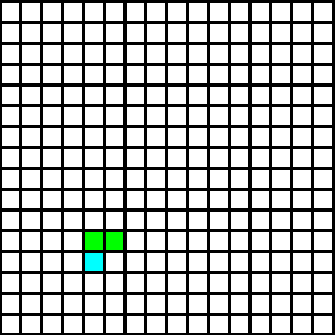
\includegraphics[width=0.9\textwidth]{replicator-1/01}
        \caption{Step 1}
    \end{subfigure}
    \begin{subfigure}{0.32\textwidth}
        \centering
        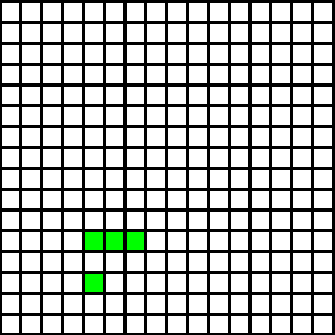
\includegraphics[width=0.9\textwidth]{replicator-1/02}
        \caption{Step 2}
    \end{subfigure}
    \begin{subfigure}{0.32\textwidth}
        \centering
        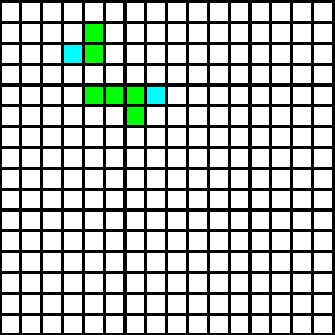
\includegraphics[width=0.9\textwidth]{replicator-1/03}
        \caption{Step 3}
    \end{subfigure}
    \begin{subfigure}{0.32\textwidth}
        \centering
        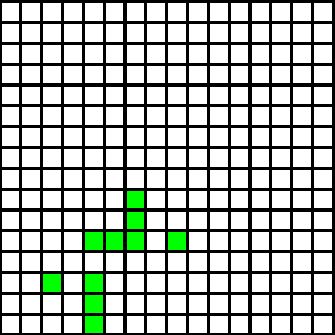
\includegraphics[width=0.9\textwidth]{replicator-1/04}
        \caption{Step 4}
    \end{subfigure}
    \begin{subfigure}{0.32\textwidth}
        \centering
        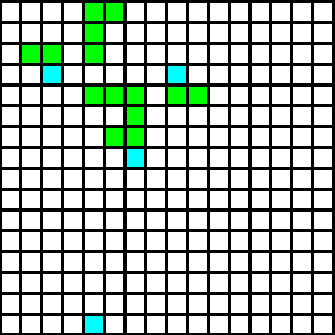
\includegraphics[width=0.9\textwidth]{replicator-1/05}
        \caption{Step 5}
    \end{subfigure}
    \begin{subfigure}{0.32\textwidth}
        \centering
        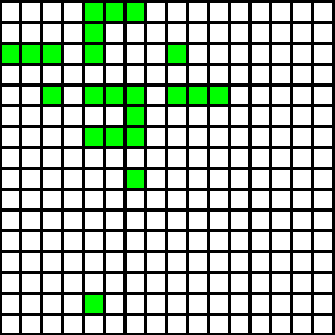
\includegraphics[width=0.9\textwidth]{replicator-1/06}
        \caption{Step 6}
    \end{subfigure}
    \begin{subfigure}{0.32\textwidth}
        \centering
        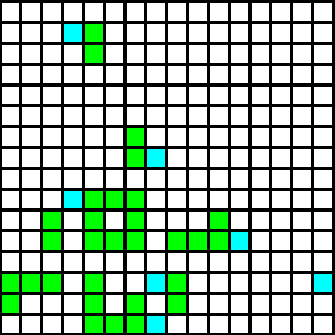
\includegraphics[width=0.9\textwidth]{replicator-1/07}
        \caption{Step 7}
    \end{subfigure}
    \begin{subfigure}{0.32\textwidth}
        \centering
        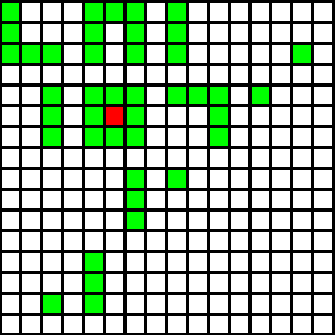
\includegraphics[width=0.9\textwidth]{replicator-1/08}
        \caption{Step 8}
    \end{subfigure}
    \begin{subfigure}{0.32\textwidth}
        \centering
        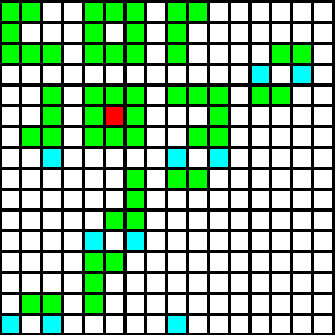
\includegraphics[width=0.9\textwidth]{replicator-1/09}
        \caption{Step 9}
    \end{subfigure}
    \begin{subfigure}{0.32\textwidth}
        \centering
        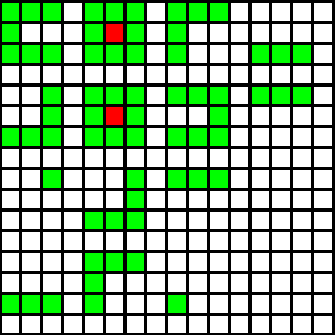
\includegraphics[width=0.9\textwidth]{replicator-1/10}
        \caption{Step 10}
    \end{subfigure}
    \begin{subfigure}{0.32\textwidth}
        \centering
        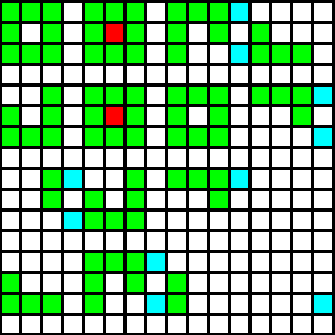
\includegraphics[width=0.9\textwidth]{replicator-1/11}
        \caption{Step 11}
    \end{subfigure}
\end{figure}

\begin{figure}[!ht]
    \ContinuedFloat
    \centering
    \begin{subfigure}{0.32\textwidth}
        \centering
        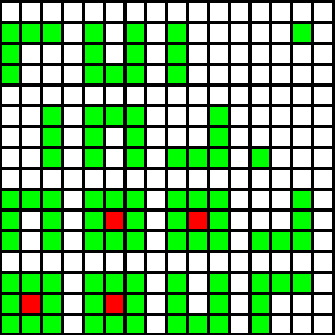
\includegraphics[width=0.9\textwidth]{replicator-1/12}
        \caption{Step 12}
    \end{subfigure}
    \begin{subfigure}{0.32\textwidth}
        \centering
        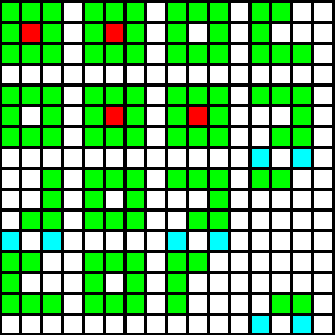
\includegraphics[width=0.9\textwidth]{replicator-1/13}
        \caption{Step 13}
    \end{subfigure}
    \begin{subfigure}{0.32\textwidth}
        \centering
        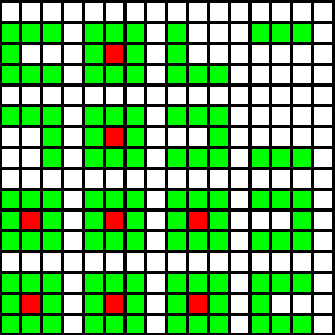
\includegraphics[width=0.9\textwidth]{replicator-1/14}
        \caption{Step 14}
    \end{subfigure}
    \begin{subfigure}{0.32\textwidth}
        \centering
        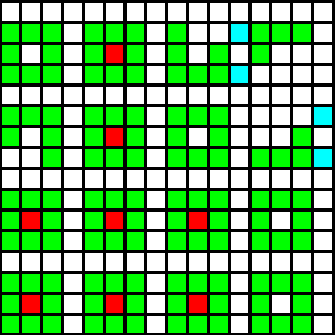
\includegraphics[width=0.9\textwidth]{replicator-1/15}
        \caption{Step 15}
    \end{subfigure}
    \begin{subfigure}{0.32\textwidth}
        \centering
        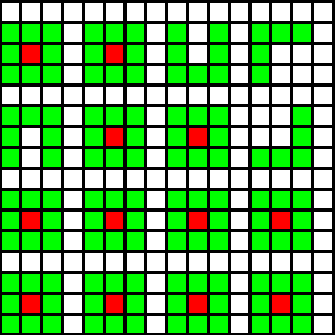
\includegraphics[width=0.9\textwidth]{replicator-1/16}
        \caption{Step 16}
    \end{subfigure}
    \begin{subfigure}{0.32\textwidth}
        \centering
        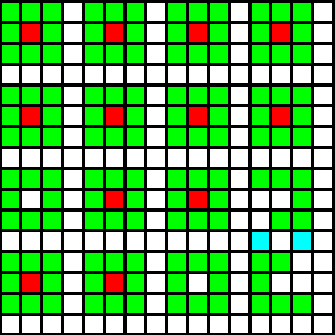
\includegraphics[width=0.9\textwidth]{replicator-1/17}
        \caption{Step 17}
    \end{subfigure}
    \begin{subfigure}{0.32\textwidth}
        \centering
        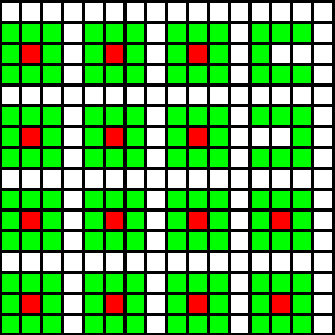
\includegraphics[width=0.9\textwidth]{replicator-1/18}
        \caption{Step 18}
    \end{subfigure}
    \begin{subfigure}{0.32\textwidth}
        \centering
        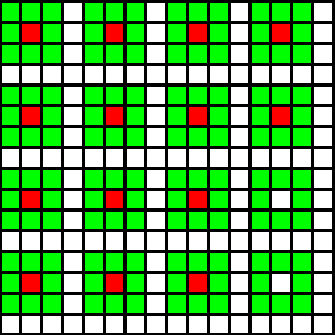
\includegraphics[width=0.9\textwidth]{replicator-1/19}
        \caption{Step 19}
    \end{subfigure}
    \begin{subfigure}{0.32\textwidth}
        \centering
        \includegraphics[width=0.9\textwidth]{replicator-1/20}
        \caption{Step 20}
    \end{subfigure}
    \caption[Replicator 1] {
        TODO
    }
    \label{fig:replicator-1}
\end{figure}


\chapter{Discussion}
    \label{ch:discussion}
    \TODO

\section{Warnings}

\begin{itemize}
    \item Most are due to parameterization
    \item Many from generated PCIE core
    \item Nearly all filtered to make output more readable and make it easier to find bugs
    \item Could not remove remaining due to limited filter system (don't want to cause trouble later)
    \item 728 in ISE (684 filtered)
    \item 502 in XST (457 filtered)
    \item Why the difference?
    \item Also filtered "equivalent register removal" infos to reduce clutter
\end{itemize}


\chapter{Conclusion}
    \label{ch:conclusion}
    In this paper, NTNU's CA research platform has been completely re-engineered.
The overall structure is equivalent, but the hardware design has been made more modular, configurable and structured, and the software API more adaptable, complete and user-friendly.
The 2D and 3D designs have been unified and any external dependencies removed.

It has been thoroughly tested in hardware and solves nearly all issues with the previous design.
There are however some issues with the communication module, which is ironic as its implementation was the original task of the project.
However, when the design is restored to 125 MHz, the raw CA performance should be 35\% higher in 2D and about 300\% higher in 3D at lower or equivalent resource usage.

In essence, this thesis provides a complete tool for CA research and experimentation.
It allows study of self-organization, adaptation and... \TODO

It can be integrated into any system with a recent version of Linux and an available PCI Express socked.

\todo{remove these notes}
Complete tool for CA research.
Tried and tested (examples).
Good performance.
Should be easily extendable for larger FPGAs.
Can be integrated into current systems.
Research platform for self-org, adaptation, ++
List use cases.
Thoroughly tested.


\cleardoublepage
\phantomsection
\addcontentsline{toc}{chapter}{Bibliography}
\bibliographystyle{plain}
\bibliography{references}

\appendix

\chapter{Test Descriptions}
    \label{app:test-descriptions}
    \begin{table}[!ht]
    \renewcommand{\arraystretch}{1.4}
    \centering
    \begin{tabularx}{\textwidth}{c|>{\raggedright\arraybackslash}X|>{\raggedright\arraybackslash}p{0.25\textwidth}}
        \bfseries Test & \bfseries Description & \bfseries Verifies \\
        \hline
        0 & Write types one by one, read them, check that types match & Write~One~Type, Read~One~Type \\
        1 & Write types row by row, read all, check that types match & Write~Row~Types, Read~All~Types \\
        2 & Write states one by one, read them, check that states match & Write~One~State, Read~One~State \\
        3 & Write states row by row, read all, check that states match & Write~Row~States, Read~All~States \\
        4 & Fill cells, check that all cells have correct type and state & Fill Cells \\
        5 & Write states and types, swap, check that data is gone, swap again, check that data is back & Swap~Cell~Storage \\
        6 & Write rules and types, develop, check rules have triggered and types have updated & Develop, Write~Rule, Read~Rule~Vectors, Read~Rule~Numbers \\
        7 & Write states, configure the sblock matrix, read it back, check that states are unchanged & Config, Readback \\
        8 & Write states, types and LUTs, configure sblock matrix, check states have changed & Step, Write~LUT \\
        9 & Store program that sends 1 and then stops, jump to program address three times, check for three 1s & Store, End, Jump, Break \\
        10 & Execute program that sends 1, increments counter and jumps to itself unless the counter is equal to three, check for three 1s & Jump~Equal, Counter~Reset, Counter~Increment \\
    \end{tabularx}
\end{table}



\chapter{Attached Files}
    \label{app:attached-files}
    An archive containing the code for the hardware design and the software API should be distributed with this thesis.
If not, all resources related to the project can be found online at \url{https://github.com/lundal/carp}.

Nearly all files from previous designs have been completely discarded, but parts of old code have been reused in a few places.

\section*{Directory Structure}

\dirtree{%
.1 attachment.zip.
    .2 api.
        .3 libcarp.
        .3 programs.
    .2 vhdl.
        .3 ipcores.
        .3 modules.
            .4 cellular\_automata.
            .4 communication.
            .4 development.
            .4 fetch.
            .4 fitness.
            .4 utility.
        .3 packages.
        .3 sp605.
        .3 testbenches.
}

\clearpage
\section*{API Files}

\dirtree{%
.1 api.
    .2 makefile \DTcomment{Build script}.
}
~
\dirtree{%
.1 api/libcarp.
    .2 bitvector.[c|h] \DTcomment{Utility bit string builder}.
    .2 carp.[c|h] \DTcomment{Main API}.
    .2 communication.[c|h] \DTcomment{Communication module interface}.
    .2 instructions.h \DTcomment{Instruction code definitions}.
    .2 lut.h \DTcomment{LUT data structure}.
    .2 matrix.[c|h] \DTcomment{Matrix data structure}.
    .2 pci.[c|h] \DTcomment{Generic PCI/PCI Express interface}.
    .2 postscript.[c|h] \DTcomment{Optional PostScript API}.
    .2 print.[c|h] \DTcomment{Optional print API}.
    .2 rule.h \DTcomment{Development rule data structure}.
    .2 utility.[c|h] \DTcomment{Various utility functions}.
}
~
\dirtree{%
.1 api/programs.
    .2 demo\_development.c \DTcomment{Simple development example}.
    .2 demo\_replicator.c \DTcomment{Simple replicator example}.
    .2 demo\_stacked.c \DTcomment{Simple stacked-mode example}.
    .2 profile\_communication.c \DTcomment{Profiles latency and throughput}.
    .2 test\_config\_readback.c \DTcomment{Test 7}.
    .2 test\_counters.c \DTcomment{Test 10}.
    .2 test\_development.c \DTcomment{Test 6}.
    .2 test\_fill\_cells.c \DTcomment{Test 4}.
    .2 test\_instructions\_storage.c \DTcomment{Test 9}.
    .2 test\_sblockmatrix.c \DTcomment{Test 8}.
    .2 test\_swap\_cell\_storage.c \DTcomment{Test 5}.
    .2 test\_write\_read\_state.c \DTcomment{Test 2}.
    .2 test\_write\_read\_states.c \DTcomment{Test 3}.
    .2 test\_write\_read\_type.c \DTcomment{Test 0}.
    .2 test\_write\_read\_types.c \DTcomment{Test 1}.
    .2 testframework.cinclude \DTcomment{Framework used by all tests}.
}

\clearpage
\section*{VHDL Files}

\dirtree{%
.1 vhdl.
    .2 carp.xise \DTcomment{ISE project file}.
    .2 filter.filter \DTcomment{Warning filter rules}.
    .2 makefile \DTcomment{Build script}.
    .2 parameters.conf \DTcomment{Synthesis parameters}.
}
~
\dirtree{%
.1 vhdl/ipcores.
    .2 sp605\_pcie.xco \DTcomment{PCI Express IP core configuration}.
}
~
\dirtree{%
.1 vhdl/modules.
    .2 cell\_storage.vhd \DTcomment{Cell Storage}.
    .2 cell\_storage\_mux.vhd \DTcomment{Cell Storage Multiplexer}.
    .2 cell\_writer\_reader.vhd \DTcomment{Cell Writer Reader}.
    .2 decode.vhd \DTcomment{Decode}.
    .2 fitness\_sender.vhd \DTcomment{Fitness Sender}.
    .2 information\_sender.vhd \DTcomment{Information Sender}.
    .2 lut\_writer.vhd \DTcomment{LUT Writer}.
    .2 resetter.vhd \DTcomment{Buffer Resetter}.
    .2 rule\_numbers\_reader.vhd \DTcomment{Rule Numbers Reader}.
    .2 rule\_vector\_reader.vhd \DTcomment{Rule Vector Reader}.
    .2 rule\_writer.vhd \DTcomment{Rule Writer}.
    .2 send\_buffer\_mux.vhd \DTcomment{Send Buffer Multiplexer}.
    .2 toplevel.vhd.in \DTcomment{Toplevel; preprocessed to toplevel.vhd}.
}
~
\dirtree{%
.1 vhdl/modules/cellular\_automata.
    .2 cellular\_automata.vhd \DTcomment{Cellular Automaton}.
    .2 live\_counter.vhd \DTcomment{Live Counter}.
    .2 lut\_configurable.vhd \DTcomment{Configurable LUT}.
    .2 sblock.vhd \DTcomment{Single sblock}.
    .2 sblock\_matrix.vhd \DTcomment{Sblock Matrix}.
}
~
\dirtree{%
.1 vhdl/modules/communication.
    .2 communication.vhd \DTcomment{PCI Express communication module}.
    .2 communication\_sim.vhd \DTcomment{Simulation version which exposes buffers}.
    .2 rq\_special.vhd \DTcomment{Special Request Handler}.
    .2 rx\_engine.vhd \DTcomment{Reception Engine: Parses TLPs}.
    .2 tx\_engine.vhd \DTcomment{Transmission Engine: Builds TLPs}.
}
\clearpage
\dirtree{%
.1 vhdl/modules/development.
    .2 cell\_fetcher.vhd \DTcomment{Cell Fetcher}.
    .2 development.vhd \DTcomment{Development}.
    .2 hits\_to\_numbers.vhd \DTcomment{Hits To Numbers processor}.
    .2 hits\_to\_vector.vhd \DTcomment{Hits To Vector processor}.
    .2 rule\_fetcher.vhd \DTcomment{Rule Fetcher}.
    .2 rule\_tester.vhd \DTcomment{Single-rule Rule Tester}.
    .2 rule\_tester\_multi.vhd \DTcomment{Multi-rule Rule Tester}.
    .2 rule\_testers\_multi.vhd \DTcomment{Multiple multi-rule Rule Testers}.
}
~
\dirtree{%
.1 vhdl/modules/fetch.
    .2 fetch.vhd \DTcomment{Fetch}.
    .2 fetch\_communication.vhd \DTcomment{Fetch Communication}.
    .2 fetch\_handler.vhd \DTcomment{Fetch Handler}.
}
~
\dirtree{%
.1 vhdl/modules/fitness.
    .2 dft.vhd \DTcomment{DFT}.
    .2 dsp\_wrapper.vhd \DTcomment{DSP Wrapper}.
    .2 fitness\_dft.vhd \DTcomment{DFT Fitness}.
    .2 fitness\_live\_counter.vhd \DTcomment{Live Count Fitness}.
    .2 twiddles.vhd \DTcomment{DFT twiddle factors generator}.
}
~
\dirtree{%
.1 vhdl/modules/utility.
    .2 bit\_counter\_32.vhd \DTcomment{Counts number of ones in 32 bits}.
    .2 bit\_counter\_N.vhd \DTcomment{Counts number of ones in N bits}.
    .2 bram\_1toN.vhd \DTcomment{1-in N-out BRAM}.
    .2 bram\_tdp.vhd \DTcomment{Dual-port BRAM}.
    .2 combiner.vhd \DTcomment{Combiner}.
    .2 fifo.vhd \DTcomment{FIFO}.
    .2 selector.vhd \DTcomment{Selector}.
    .2 shifter.vhd \DTcomment{Static shifter}.
    .2 shifter\_dynamic.vhd \DTcomment{Dynamic shifter}.
    .2 shift\_register.vhd \DTcomment{Shift register}.
}
~
\dirtree{%
.1 vhdl/packages.
    .2 functions.vhd \DTcomment{Utility functions}.
    .2 instructions.vhd \DTcomment{Instruction codes}.
    .2 types.vhd \DTcomment{Custom type declarations}.
}
~
\dirtree{%
.1 vhdl/sp605.
    .2 constraints.ucf.in \DTcomment{Constraints; preprocessed to constraints.ucf}.
    .2 pcie\_wrapper.vhd \DTcomment{PCI Express Endpoint Core wrapper}.
}
~
\dirtree{%
.1 vhdl/testbenches.
    .2 test\_template.vhd \DTcomment{Testbench template}.
    .2 test\_dft.vhd \DTcomment{DFT testbench}.
    .2 test\_dsp\_wrapper.vhd \DTcomment{DSP Wrapper testbench}.
}


\chapter{Instruction Set Architecture}
    \label{app:isa}
    \cleardoublepage
    \includepdf[pages={3-}]{includes/isa.pdf}

\chapter{Specialization Project Report}
    \label{app:specialization-project}
    \cleardoublepage
    \includepdf[pages={-}]{includes/report.pdf}

\end{document}
